\documentclass[11pt,ngerman]{article}
\usepackage{geometry}
\usepackage[T1]{fontenc}
\usepackage[utf8]{inputenc}
\usepackage{babel}
\usepackage{lmodern}%get scalable font
\usepackage{titling}
\usepackage{relsize}
\usepackage{biblatex}
\usepackage{hyperref}
\usepackage[toc]{glossaries}
\usepackage{paralist}
\usepackage[table, dvipsnames]{xcolor}
\usepackage{booktabs}
\usepackage{tabularx}
\usepackage{float}
\restylefloat{table}
\usepackage{setspace}
\usepackage{multicol}
\usepackage{graphicx}
\usepackage[space]{grffile}
\usepackage[most]{tcolorbox}
\usepackage{enumitem}
\usepackage{textcomp}
\usepackage{listings}
\usepackage[flushleft]{threeparttable}

% Document geometry
\geometry{a4paper, top=25mm, left=25mm, right=25mm, bottom=20mm,
    headsep=10mm, footskip=12mm}

% Link colors
\hypersetup{
    colorlinks,
    linkcolor={blue},
    citecolor={red},
    urlcolor={blue}
}

% double quotes macro
% usage: \quotes{arg1}  => in text: "arg1"
\newcommand{\quotes}[1]{``#1''}

% inline code macro
\definecolor{lightgray}{gray}{0.9}
\lstset{
    showstringspaces=false,
    basicstyle=\ttfamily,
    keywordstyle=\color{blue},
    commentstyle=\color[grey]{0.6},
    stringstyle=\color[RGB]{255,150,75}
}
\newcommand{\inlinecode}[2]{\colorbox{lightgray}{\lstinline[language=#1]$#2$}}

% Code block settings
\definecolor{codegreen}{rgb}{0,0.6,0}
\definecolor{codegray}{rgb}{0.5,0.5,0.5}
\definecolor{codepurple}{rgb}{0.58,0,0.82}
\definecolor{backcolour}{rgb}{0.95,0.95,0.92}

\lstdefinestyle{mystyle}{
    backgroundcolor=\color{backcolour},
    commentstyle=\color{codegreen},
    keywordstyle=\color{magenta},
    numberstyle=\tiny\color{codegray},
    stringstyle=\color{codepurple},
    basicstyle=\ttfamily\footnotesize,
    breakatwhitespace=false,
    breaklines=true,
    captionpos=b,
    keepspaces=true,
    numbers=left,
    numbersep=5pt,
    showspaces=false,
    showstringspaces=false,
    showtabs=false,
    tabsize=2
}
\lstset{style=mystyle}

% Glossary
% Das Glossar definiert alle wichtigen Begriffe zur Sicherstellung einer einheitlichen Terminologie.
% Es sollen keine allgemeinen Begriffe erklärt werden, die den Adressaten bekannt sind (z. B. Java, CPU etc.).
% Glossareinträge müssen im Text verwendet werden, damit diese im Glossar im Appendix \printglossary angezeigt werden
\makeglossaries
\loadglsentries{glossary} % loads glossary definitions from external file


% bibliography file
\addbibresource{\jobname.bib}

% pre-, post title setting
\pretitle{\begin{center}\linespread{1.5}\huge}
    \posttitle{\par\end{center}\vspace{0.5em}}

\begin{document}

    \title{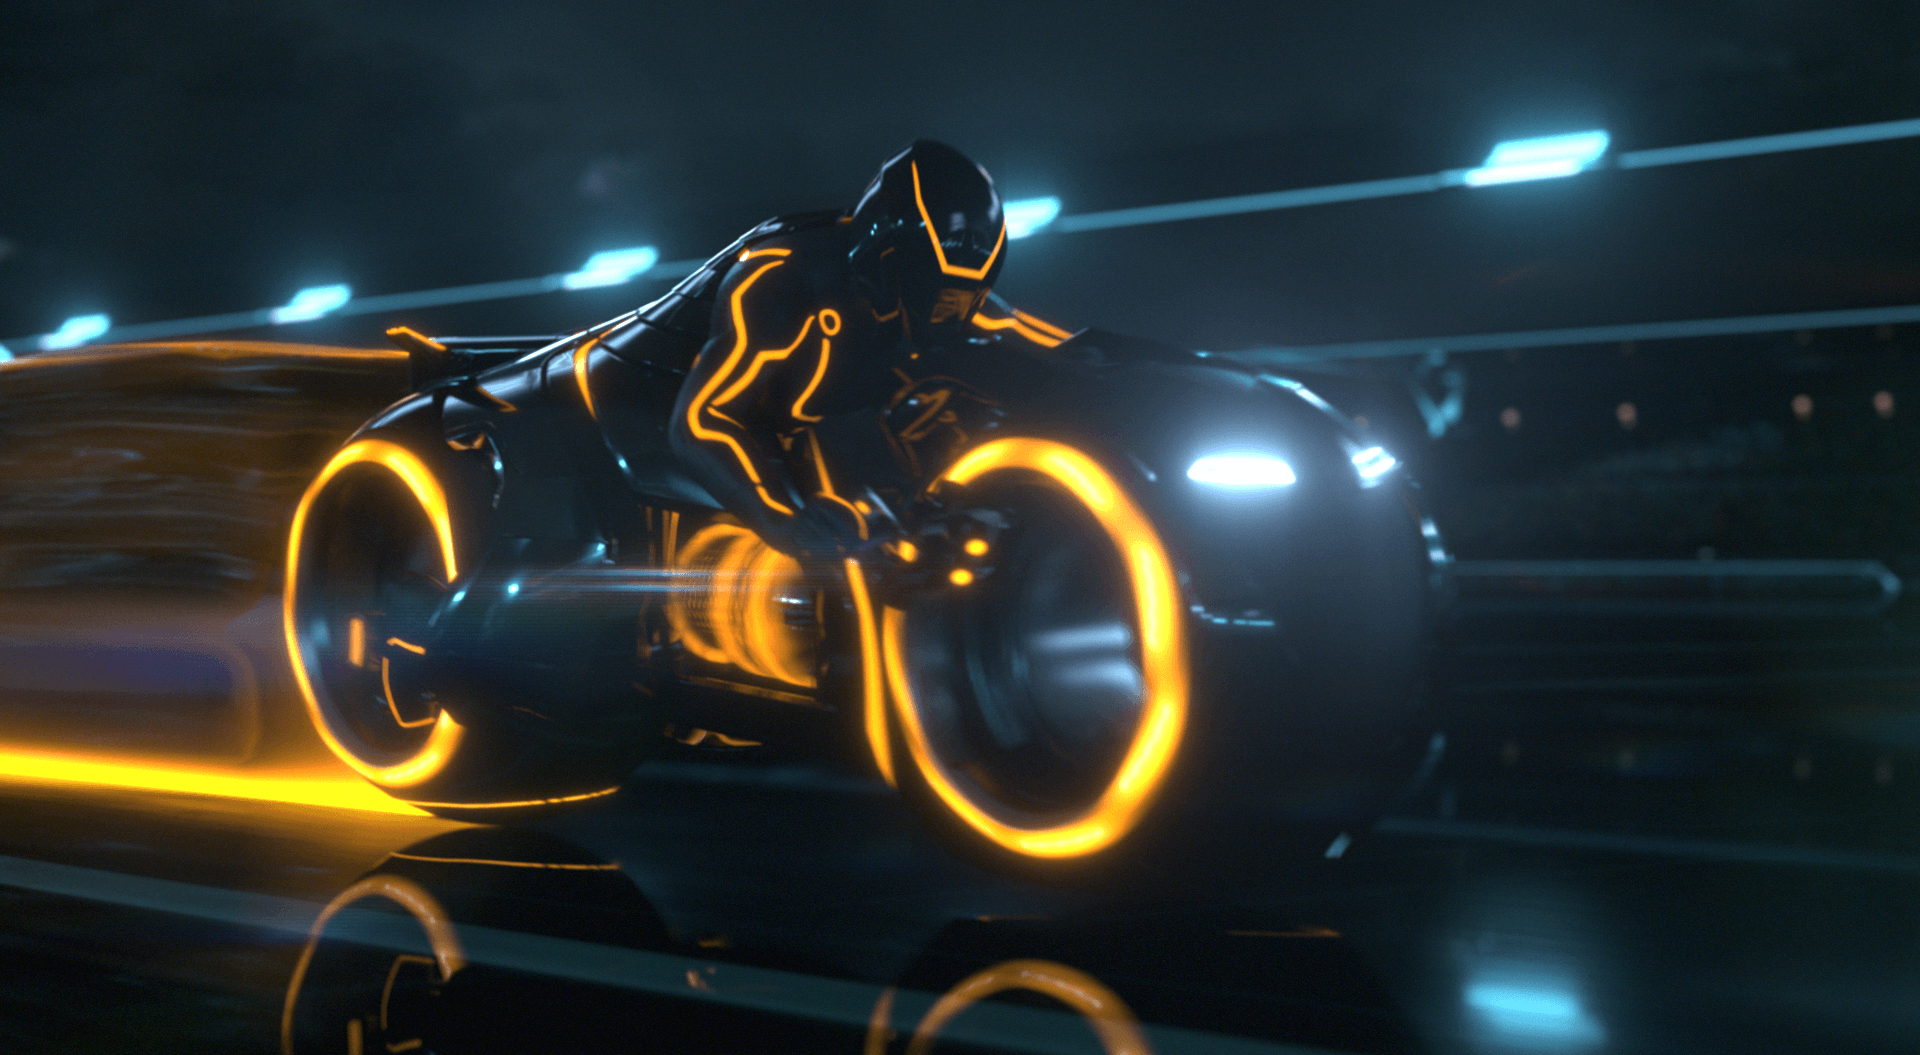
\includegraphics[width=1\textwidth]{figures/Tron-Legacy_Bike.png}\\ Tron Licht-Motorräder Computerspiel\\
        \vspace{1cm}
        \smaller{}Schlussbericht \\
        \vspace{0.5cm}
        \small{}ZHAW  School of Engineering
        \vspace{1.5cm}
    }
    \author{
        Akca, Deniz\\
        \small{akcaden1@students.zhaw.ch}
        \and
        Holenstein, Christian\\
        \small{holenchr@students.zhaw.ch}
        \and
        Huber, Patrick\\
        \small{huberpa4@students.zhaw.ch}
        \and
        Iten, Mike\\
        \small{itenmik1@students.zhaw.ch}
        \vspace{1.5cm}
    }
   \date{\today}

    \maketitle
    \newpage

    \tableofcontents
    \newpage

%%% Projektidee
    \section{Projektidee}

    \subsection{Ursprüngliche Idee}
    Es soll ein netzwerkfähiges und browserbasiertes Tron-Spiel entwickelt werden, genauer gesagt die Version mit den  Licht-Motorrädern. Das Spiel soll eine ansprechende und simple Benutzeroberfläche besitzen sodass schnell und einfach gespielt werden kann. Das Spiel wird im \Gls{Multiplayer}-Modus angeboten. Ein Spieler wird gegen ihm bekannte oder unbekannte Spieler antreten können.

    \subsubsection{Original Tron}
    1982 wurde der Film "Tron"\ von Steven Lisberger ausgestrahlt, der grosse Beliebtheit erlangte \cite{lisbergerTRON1982}\cite{TronFilm2020}. Danach wurden verschiedene Spielversionen von Tron produziert. Unter anderem auch eine Version mit Licht-Motorrädern die gegeneinander antreten müssen.

    \subsubsection{Spielbeschreibung}
    Ein Spieler besitzt ein sogenanntes Licht-Motorrad. Dieses zieht während der Fahrt eine Linie nach sich, die bestehen bleibt. Fährt ein Spieler in eine dieser Linien, scheidet dieser aus. Gewinner ist, wer im Spiel bleibt, bis alle anderen Spieler ausgeschieden sind.

    \subsection{Kundennutzen}
    In der Pause während der Arbeit oder als sonstiger Zeitvertreib, versüsst unser Spiel den Alltag des Anwenders. Es besticht durch seine Einfachheit. Dies führt dazu, dass die Konzentration des Spielers voll und ganz auf das Spiel selbst gelenkt ist und er dieses in vollen Zügen geniessen kann. Danach wird er erholt zu seinen täglichen Aufgaben zurückkehren. Über ein Gastkonto ist es einem Spieler möglich, ohne jegliche Registrierung, sofort zu spielen. Möchte ein Spieler seine Fortschritte gespeichert und abrufbar haben, kann er einen Account einrichten. Die gespeicherten Punkte dienen dann als Indiz für die Applikation, um den Spieler gegen ähnlich starke Gegner antreten zu lassen. Ausserdem kann das Spiel mit Freunden gespielt werden. Ein spannender Feierabend oder Samstagnachmittag - reich an sozialer Interaktion - ist garantiert.
    Es gibt reichlich weitere Features, die gegebenenfalls implementiert werden können (siehe \ref{Weiterführende Ideen}), um kontinuierlichen Spielspass gewährleisten zu können.

    \subsection{Stand der Technik / Konkurrenzanalyse}
    Es gibt mehrere kostenlose Onlinespiele, welche im Browser gespielt werden können. \Gls{Multiplayer} ist teilweise möglich. Mindestens Drei dieser Tron-Spiele können ebenfalls über das Netzwerk (\Gls{Game Server}) gespielt werden. \cite{TronGameBasisKostenlosOnline}\cite{sphinxCyclewarsIoOnline}\cite{TronLightCyclesEu}\cite{PlayersOnlineXtremeTron}
    Viele der vorhandenen Spiele nutzen veraltete Technologien wie den \Gls{Adobe Flash Player} \cite{SayingGoodbyeFlash2017}\cite{FlashFutureInteractive2017} und nicht mehr zeitgemässe Grafiken. Ausserdem sind die grafischen Oberflächen häufig schwer verständlich.
    Momentan sind zwei moderne Tron Spiele auf dem Markt, die sich jedoch nicht nur auf das Fahren von Licht-Motorrädern beschränken. Vielmehr handelt es sich dabei um komplexe Action Spiele in 3-D Grafik, jeweils mit geführter Storyline.\cite{TronEvolution2020}\cite{TRONRUNr}

    \subsection{Hauptablauf (Kontextszenario)}

    \subsubsection{Anwender-Identifikation/-Verifikation}
	Der Anwender meldet sich anonym als Gast in der Applikation an oder loggt sich mit einem bestehenden Account ein. Um in ein Spiel zu gelangen, kann der Anwender entscheiden, ob er eine Lobby erstellen oder einer bestehenden Lobby beitreten möchten.

	\subsubsection{\Gls{Lobby} erstellen}
	Falls der Anwender eine Lobby erstellt, kann er auswählen ob diese nur für ausgewählte Spieler sichtbar ist oder jegliche Spieler beitreten können. Als Ersteller der Lobby kann der Anwender das Spiel starten, wenn alle anderen Spieler in der Lobby den Status auf 'bereit' gewechselt haben.

	\subsubsection{\Gls{Lobby} beitreten}
	Falls der Anwender einer Lobby beitreten möchte, kann er sich eine gewünschte Lobby aus der Lobby-Liste aussuchen. Als Nicht-Ersteller der Lobby kann der Status auf 'bereit' gewechselt und auf den Start des Spiels gewartet werden.

	\subsubsection{Spielstart und Rangliste}
	Die Anwendung wechselt zur \Gls{Arena} und das Spiel beginnt. Der Anwender spielt 5 Runden. Am Ende der 5 Runden zeigt die Anwendung dem Anwender die Rangliste an.

    \subsection{Ressourcen}
    Das Projekt ist realisierbar mit einem Team aus 4 Personen. Grundlegendes Wissen im Bereich der Server-Client-Kommunikation ist notwendig, sowie Kenntnisse von objektorientierter Programmierung (\Gls{OOP}), Java und Javascript. Dieses Wissen ist im Team vorhanden. Des Weiteren bestehen Kenntnisse zum Web-Design mit React, HTML5 und CSS3.
    Der Gesamtaufwand für das finale Spiel mit Basisfunktionen und Original-Spielmodus wird auf ca. 500 - 600 Stunden geschätzt. Dies entspricht ungefähr 138 Stunden Aufwand pro Person.

    \subsection{Wirtschaftlichkeit}

    \subsubsection{Aufwand erste Version}
    Um die erste, initiale, über das Netzwerk (\Gls{Game Server}) spielbare Version fertigzustellen, rechnen wir mit folgendem Aufwand. \\
    \\
    Kalkulationsformel:
        \begin{center}
            \begin{itshape}
                Projektplanung + Entwicklung + Dokumentation/Testing/Deployment = \\
                \vspace{0.5em}
                2 Wochen * 1.5 Arbeitstage * 4 Mitarbeiter * 8 Arbeitsstunden + \\
                \vspace{0.5em}
                9 Wochen * 1.5 Arbeitstage * 4 Mitarbeiter * 8 Arbeitsstunden + \\
                \vspace{0.5em}
                1 Woche * 1.5 Arbeitstage * 4 Mitarbeiter * 8 Arbeitsstunden \\
                \vspace{0.5em}
                \textbf{= 576 Arbeitsstunden}
            \end{itshape}
        \end{center}

    \subsubsection{Werbung als Einnahmequelle}
    Einnahmen werden hauptsächlich durch Werbeanzeigen generiert. Genaue Berechnungen bezüglich der Einnahmen gestallten sich als relativ schwierig, da sich die Besucheranzahl auf der Webseite über die Zeit ändern kann. Ausserdem sind die Einnahmen abhängig von der Bezahlstrategie und davon, wie stark der Inhalt der angezeigten Werbung den jeweiligen Webseitenbesucher anspricht\cite{CPCVsCPA2019}\cite{daswani2008online}. \\
    \\
    Berechnung nach Google Adsense Calculator \cite{GoogleAdSenseEarn}:
    \begin{center}
        \begin{tabular}{ | l | l | l | p{5cm} |}
            \hline
            Monthly page views & Monthly revenue [\$]  \\ \hline
            500'000 & 1'925 \\ \hline
            1'000'000 & 3'850 \\ \hline
            2'500'000 & 9'625 \\ \hline
            5'000'000 & 19'250 \\ \hline
            10'000'000 & 38'500 \\ \hline
        \end{tabular}
    \end{center}

    \subsubsection{Return of Invest}
    Die geschätzte initiale Investition beträgt bei 576 Arbeitsstunden Aufwand und einem Stundensatz von 50.- pro Stunde plus einer kleinen Reserve für zusätzliche Ausgaben:
    \[576\ h * 50.- + 5'000 = 33'800\ CHF\]
    Die Einnahmen bei 2'500'000 monatlichen Besuchern (Laden der Webseite)  würden sich auf monatlich 9'625 CHF belaufen. Wenn wir die monatlichen Kosten für den Webseitenbetrieb vernachlässigen, hätten wir nach ca. 4 Monaten die Entwicklungskosten amortisiert    .\\
% END Projektidee

    \newpage

%%% Analyse
    \section{Analyse}

    \subsection{Anwendungsfälle}
    Die in \autoref{fig:UseCaseDiagram} ersichtlichen Anwendungsfälle sind hier nach Priorität geordnet aufgelistet:
    \begin{multicols}{2}
    	\begin{itemize}
    		\item  \hyperref[ssec:UC1Lobbyerstellen]{UC1: Lobby erstellen - \quotes{fully dressed}}
    		\item\hyperref[ssec:UC2Spielspielen]{UC2: Spiel spielen - \quotes{fully dressed}}
    		\item \hyperref[sssec:UC3EinAusloggen]{UC3: Ein \& Ausloggen  - \quotes{casual}}
    		\item \hyperref[sssec:UC4Lobbybeitreten]{UC4: Lobby beitreten - \quotes{casual}}
    		\item \hyperref[sssec:UC5Registrieren]{UC5: Registrieren - \quotes{brief}}
    		\item \hyperref[sssec:UC6Passwortsetzen]{UC6: Passwort zurücksetzen - \quotes{brief}}
    		\item  \hyperref[sssec:UC7Spielereinladen]{UC7: Spieler einladen - \quotes{brief}}
    		\item \hyperref[sssec:UC8Statistikenbetrachten]{UC8: Statistiken betrachten - \quotes{brief}}
    	\end{itemize}
    \end{multicols}

    \subsubsection{Anwendungsfalldiagramm}
    \begin{figure}[H]
    	\centering
    	\makebox[\textwidth][c]{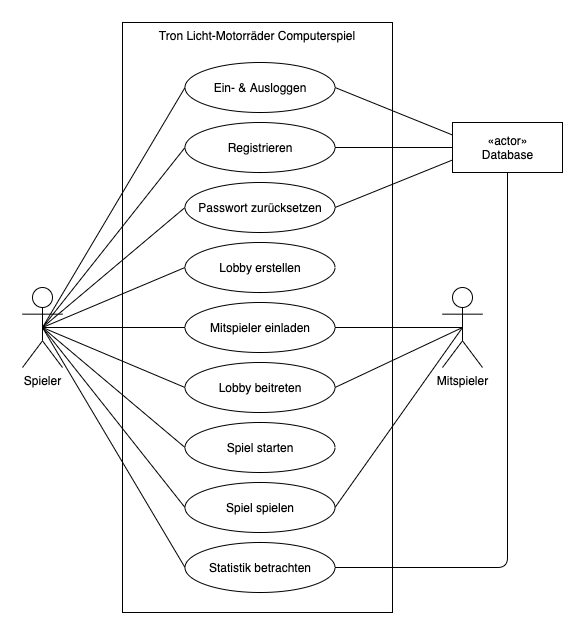
\includegraphics[width=0.9\textwidth]{figures/Use-case-modell.png}}
    	\caption{Anwendungsfalldiagramm - Tron Licht-Motorräder Computerspiel}
    	\label{fig:UseCaseDiagram}
    \end{figure}

    \subsubsection{Hauptanwendungsfälle}
    \label{ssec:Hauptanwendungsfaelle}
    Wir haben zwei Hauptanwendungsfälle identifiziert:
    \begin{itemize}
    	\item  \hyperref[ssec:UC1Lobbyerstellen]{UC1: Lobby erstellen - \quotes{fully dressed}}
    	\item\hyperref[ssec:UC2Spielspielen]{UC2: Spiel spielen - \quotes{fully dressed}}
    \end{itemize}
    Die Hauptanwendungsfälle werden in den nächsten zwei Abschnitten detailliert ausgeführt.

    \subsubsection{UC1: Lobby erstellen - \quotes{fully dressed}}
    \label{ssec:UC1Lobbyerstellen}
    \begin{tcolorbox}[enhanced, breakable, sharp corners, width=\dimexpr\textwidth-15mm\relax ,enlarge left by=10mm ,fontupper=\linespread{1.1}\selectfont, boxrule=1pt, title={UC1: Lobby erstellen}, colback=white, colframe=gray!22, coltitle=black]

    	\textbf{Anwendungsfall:} Lobby erstellen \\
    	\textbf{Ebene:} Anwenderziel \\
    	\textbf{Primärakteur:} Spieler \\
    	\textbf{Stakeholder und Interessen:}
    	\begin{itemize}
    		\item \textit{Spieler}: Möchte mit anderen Spielern zusammen in einer \Gls{Lobby} beitreten oder seine eigene \Gls{Lobby} erstellen. Kann die Rolle des Lobby-Erstellers haben.
    		\item \textit{Mitspieler}: Möchten mit anderen Spielern zusammen in einer \Gls{Lobby} beitreten. Kann die Rolle des Lobby-Erstellers haben.
    		\item \textit{Lobby-Ersteller}: Möchte das Spiel starten, wenn alle Spieler bereit sind.
    		\item \textit{System}: Möchte mehrere Spieler in einer \Gls{Lobby} haben, um ein Spiel starten zu können.
    	\end{itemize}
    	\textbf{Vorbedingungen:} Alle Spieler sind entweder mit einem persönlichen Konto oder einem Gastkonto angemeldet.\\
    	\textbf{Nachbedingungen:} Mehrere Spieler oder auch einzelne Spieler befinden sich in \Glspl{Lobby}. Das System ist in der Lage für mehrere \Glspl{Lobby}s mit jeweils mehreren zugehörigen Spielern Spielrunden zu starten. \\
    	\\  \textbf{Standardablauf:}
    	\begin{enumerate}
    		\item Spieler/Mitspieler wechselt zur Lobbyansicht der Anwendung.
    		\item Spieler/Mitspieler wählt eine bestehende öffentliche \Gls{Lobby} aus.
    		\item Spieler/Mitspieler tritt dieser \Gls{Lobby} bei.
    		\item Spieler und Mitspieler warten in \Gls{Lobby} auf weitere Mitspieler.
    		\item Spieler/Mitspieler klicken auf \quotes{Bereit}.
    		\item Lobby-Ersteller startet das Spiel.
    		\item System überprüft, ob alle Spieler in der \Gls{Lobby} bereit sind.
    	\end{enumerate}
    	\textit{Falls nicht alle Spieler bereit sind, muss der Lobby-Ersteller zu einem späteren Zeitpunkt nochmals Schritt 6 ausführen. Erst wenn alle Spieler bereit sind, wird mit Schritt 8 fortgefahren.}
    	\begin{enumerate}[resume]
    		\item System startet das Spiel.
    	\end{enumerate}
    	\textit{Es ist nun nicht mehr möglich dieser \Gls{Lobby} beizutreten.} \\
    	\textit{Spiel wird gespielt …, Ende des Spiels.}
    	\begin{enumerate}[resume]
    		\item System öffnet \Gls{Lobby} wieder
    	\end{enumerate}
    	\textit{Spieler/Mitspieler können einer \Gls{Lobby} beitreten. Punkt 3 bis 9 wiederholen sich, bis der Spieler sich entscheidet, das Spiel oder die \Gls{Lobby} zu verlassen.} \\
    	\\ \textbf{Erweiterungen (oder alternative Abläufe):}
    	\begin{itemize}
    		\item[2a.] Spieler können eigene \Gls{Lobby} erstellen:
    		\begin{enumerate}
    			\item Spieler klickt auf \Gls{Lobby} erstellen.
    			\item Spieler bestimmt, ob die \Gls{Lobby} öffentlich (public) oder nur für bestimmte Spieler (private) zugänglich sein soll.
    			\item System erstellt eine \Gls{Lobby}.
    			\item System fügt den Spieler als Lobby-Ersteller der \Gls{Lobby} hinzu.
    		\end{enumerate}
    		\item[2b.] Spieler können privater \Glspl{Lobby} über einen Link beitreten:
    		\begin{enumerate}
    			\item Spieler öffnet Einladung.
    			\item Spieler öffnet den Link im Browser.
    			\item System fügt Spieler der privaten \Gls{Lobby} hinzu.
    		\end{enumerate}
    		\item[4a.] Spieler können \Gls{Lobby} verlassen:
    		\begin{enumerate}
    			\item Spieler/Mitspieler verlassen \Gls{Lobby}
    		\end{enumerate}
    		\item[4b.] Spieler/Mitspieler können in der \Gls{Lobby} bleiben und weiterspielen:
    		\begin{enumerate}
    			\item Spieler/Mitspieler verlassen die \Gls{Lobby} nicht
    		\end{enumerate}
    	\end{itemize}
    	\textbf{Spezielle Anforderungen:}
    	\begin{itemize}
    		\item Sobald ein Mitspieler der \Gls{Lobby} beigetreten ist, läuft ein Timer. Falls der Timer abgelaufen ist und der Mitspieler noch nicht bestätigt hat, wird dieser automatisch abgelehnt.
    		\item Maximale Spieleranzahl muss eingehalten werden. Es gibt eine obere Grenze von Mitspielern, die durch den Spieler definiert wird.
    		\item Internationalisierung der Sprache in den Textanzeigen.
    	\end{itemize}

    \end{tcolorbox}

    \subsubsection{UC2: Spiel spielen - \quotes{fully dressed}}
    \label{ssec:UC2Spielspielen}
    \begin{tcolorbox}[enhanced, breakable, sharp corners, width=\dimexpr\textwidth-15mm\relax ,enlarge left by=10mm ,fontupper=\linespread{1.1}\selectfont, boxrule=1pt, title={UC2: Spiel spielen}, colback=white, colframe=gray!22, coltitle=black]

    	\textbf{Anwendungsfall:} Spiel spielen \\
    	\textbf{Ebene:} Anwenderziel \\
    	\textbf{Primärakteur:} Spieler \\
    	\textbf{Stakeholder und Interessen:}
    	\begin{itemize}
    		\item \textit{Spieler}: Möchte als letzter Spieler übrig bleiben
    		\item \textit{Mitspieler}: Möchte als letzter Spieler übrig bleiben.
    		\item \textit{Lobby-Ersteller}:  Möchte das Spiel starten, wenn alle Spieler bereit sind.
    		\item \textit{System}: Möchte alle Spieler, die bereit zum spielen sind, in einer \Gls{Lobby} haben, um ein Spiel starten zu können.
    	\end{itemize}
    	\textbf{Vorbedingungen:} Mindestens 2 Spieler sind im Spiel.\\
    	\textbf{Nachbedingungen:} Der letzte Spieler im Spiel wurde Sieger. Spiel wurde erfolgreich beendet. \Gls{Lobby} wird erneut angezeigt. \\
    	\\  \textbf{Standardablauf:}
    	\begin{enumerate}
    		\item System lädt Spiel.
    		\item System platziert Spieler/Mitspieler bzw. die Spielcharakteren - in möglichst entgegengesetzte Richtungen zeigend - mit einem gewissen Abstand zueinander und zum Spielfeldrand auf dem Spielfeld.
    		\item System zeigt Countdown an. Nach Ablauf des Countdowns beginnt das Spiel.
    		\item System beginnt Startbewegung der Spieler mit konstanter Geschwindigkeit in Richtung Spielfeldmitte.
    	\end{enumerate}
    	\textit{Alle Spieler/Mitspieler auf dem Spielfeld behalten die konstante Geschwindigkeit bei bis zum Ausscheiden oder Ende des Spiels.}
    	\begin{enumerate}[resume]
    		\item System erzeugt Hindernis vom Startpunkt des Spielers/Mitspielers bis zu dessen aktueller Position.
    		\item System übergibt Spieler/Mitspieler die Kontrolle des jeweiligen Spielcharakters.
    	\end{enumerate}
    	\textit{Schritt 4 - 6 folgen ohne Zeitverzögerung aufeinander.}
    	\begin{enumerate}[resume]
    		\item Spieler/Mitspieler können, durch drücken einer Pfeiltaste, die Richtung um jeweils exakt 90\textdegree\ ändern.
    		\item Das durch den Spieler/Mitspieler erzeugte Hindernis, wächst mit der Bewegung und in der jeweiligen Bewegungsrichtung.
    	\end{enumerate}
    	\textit{Das vom Spieler/Mitspieler erzeugte Hindernis, bleibt auf dem Spielfeld bestehen bis zum Ausscheiden oder Sieg des Spielers/Mitspielers, in allen folgenden Schritten.}
    	\begin{enumerate}[resume]
    		\item System koordiniert in kurzen Intervallen alle Bewegungen der Spieler/Mitspieler und überprüft deren Positionen und potentielle Kollisionen.
    	\end{enumerate}
    	\textit{System wiederholt Schritt 7 - 9 bis Kollision erkannt wird.}
    	\begin{enumerate}[resume]
    		\item System entfernt Spieler/Mitspieler, der Kollision verursacht, vom Spielfeld und zeigt eine entsprechende Meldung an.
    	\end{enumerate}
    	\textit{System wiederholt Schritt 7 - 10 bis nur noch ein einziger Spieler/Mitspieler auf dem Spielfeld übrig bleibt.}
    	\begin{enumerate}[resume]
    		\item System zeigt bei letztem Spieler/Mitspieler eine Siegesmeldung an.
    		\item System beendet das Spiel.
    		\item System zeigt die Statistiken des Spiels bei allen Spielern/Mitspielern an.
    		\item System öffnet nach Ablauf eines Timers erneut die \Gls{Lobby}.
    	\end{enumerate}

    \end{tcolorbox}

    \newpage
    \subsubsection{System-Sequenzdiagramm (SSD)}
    \label{sssec:SSDFromProjectOutline}
    Das System-Sequenzdiagramm für \quotes{Lobby erstellen} und \quotes{Spiel spielen}:
    \begin{figure}[H]
    	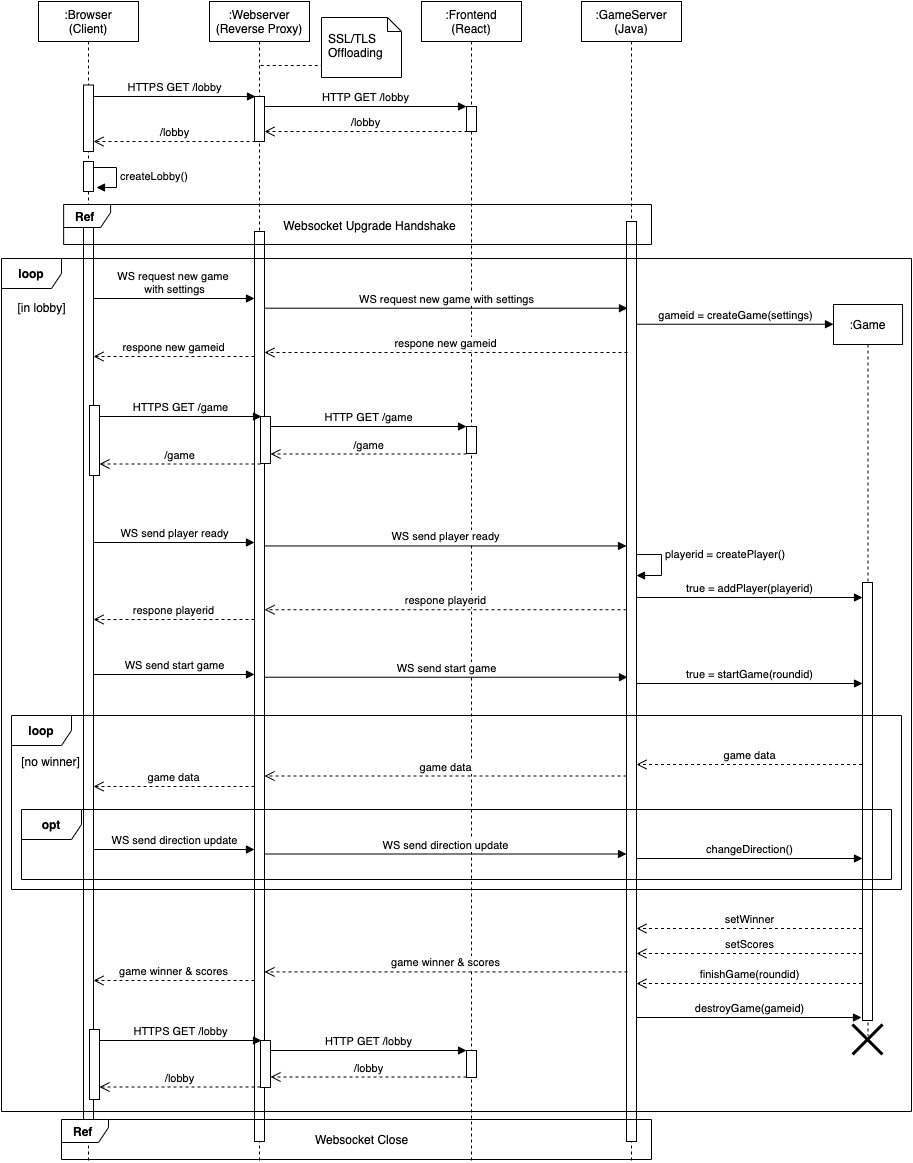
\includegraphics[scale=0.5]{figures/SystemSequenceDiagram.png}
    	\caption{System-Sequenzdiagramm - \quotes{Lobby erstellen} \&  \quotes{Spiel spielen}}
    \end{figure}
    \newpage
    \noindent \textbf{Referenz: \Gls{Websocket} Upgrade Handshake} \\
    \autoref{fig:SSDReferenzWebsocketUpgrade} zeigt den Upgrade Request der HTTP(S) Verbindung  zu \Gls{Websocket}.
    \begin{figure}[H]
    	\centering
    	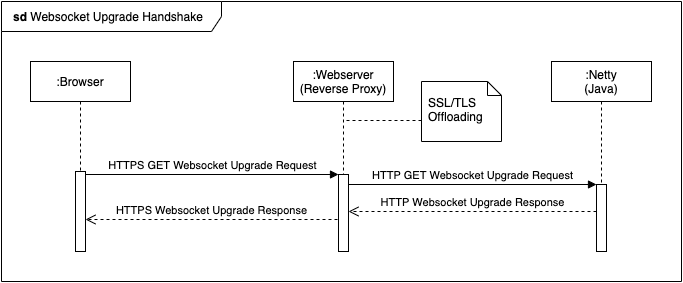
\includegraphics[scale=0.6]{figures/SSD-Websocket_Upgrade_Handshake.png}
    	\caption{SSD Referenz - \Gls{Websocket} Upgrade Handshake}
    	\label{fig:SSDReferenzWebsocketUpgrade}
    \end{figure}
    \noindent \textbf{Referenz: \Gls{Websocket} Close} \\
    \autoref{fig:SSDReferenzWebsocketClose} zeigt das schliessen der \Gls{Websocket}-Verbindung.
    \begin{figure}[H]
    	\centering
    	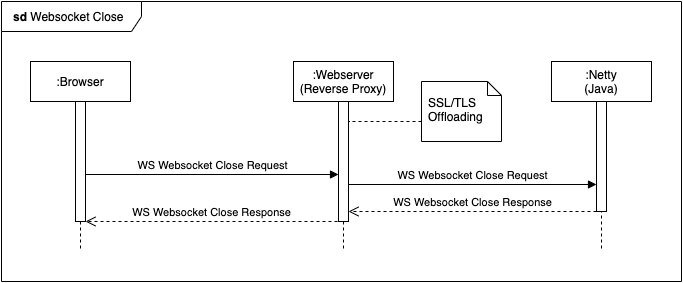
\includegraphics[scale=0.6]{figures/SSD-Websocket_Close.png}
    	\caption{SSD Referenz - \Gls{Websocket} Close}
    	\label{fig:SSDReferenzWebsocketClose}
    \end{figure}

    \subsection{Übrige Anwendungsfälle}
    \subsubsection{UC3: Ein \& Ausloggen  - \quotes{casual}}
    \label{sssec:UC3EinAusloggen}
    \begin{tcolorbox}[enhanced, breakable, sharp corners, width=\dimexpr\textwidth-15mm\relax ,enlarge left by=10mm ,fontupper=\linespread{1.1}\selectfont, boxrule=1pt, title={UC3: Ein \& Ausloggen }, colback=white, colframe=gray!22, coltitle=black]
    	\textit{Standardszenario:} Der Spieler navigiert zum Login-Bereich der Anwendung. Im Login-Bereich gibt er die korrekten Eingabedaten seines Kontos ein. Die Anwendung überprüft die Eingabedaten und meldet den Spieler an. Der
    	Spieler ist nun in der Anwendung mit seinem persönlichen Konto angemeldet.\newline
    	\newline
    	\textit{Alternative Szenarios:} \newline
    	Der Spieler gibt die falschen Eingabedaten für ein Konto ein. Das System weist den Spieler
    	daraufhin, dass die Eingabedaten falsch sind und schlägt dem Spieler vor, die Eingabedaten nocheinmal einzugeben. \newline
    	\newline
    	Der Spieler möchte sich aus dem System ausloggen. Der Spieler navigiert in der Anwendung nach oben rechts und wählt die Funktion «Logout» aus. Das System beendet die Session und der Spieler wird als Gast neu angemeldet.
    \end{tcolorbox}

    \subsubsection{UC4: Lobby beitreten - \quotes{casual}}
    \label{sssec:UC4Lobbybeitreten}
    \begin{tcolorbox}[enhanced, breakable, sharp corners, width=\dimexpr\textwidth-15mm\relax ,enlarge left by=10mm ,fontupper=\linespread{1.1}\selectfont, boxrule=1pt, title={UC4: Lobby beitreten }, colback=white, colframe=gray!22, coltitle=black]
    	\textit{Standardszenario:} Der Spieler navigiert auf der Startseite zu dem Lobbybereich, in diesem kann er einer öffentlichen Lobby beitreten. \newline
    	Nun befindet sich der Spieler in einer Lobby mit weiteren Mitspielern.\newline
    	\newline
    	\textit{Alternative Szenarios:} \newline
    	Der Spieler erhält einen Link von einem anderen Spieler, der auf eine Lobby zeigt. So kann der Spieler auch einer privaten Lobby beitreten. \newline
    \end{tcolorbox}

    \subsubsection{UC5: Registrieren - \quotes{brief}}
    \label{sssec:UC5Registrieren}
    \begin{tcolorbox}[enhanced, breakable, sharp corners, width=\dimexpr\textwidth-15mm\relax ,enlarge left by=10mm ,fontupper=\linespread{1.1}\selectfont, boxrule=1pt, title={UC5: Registrieren}, colback=white, colframe=gray!22, coltitle=black]
    	Der Spieler navigiert zum Registrier-Bereich der Anwendung. Im Registrier-Bereich gibt er den gewünschten Benutzernamen, das gewünschte Passwort und seine Email-Adresse an.\newline
    	Die Anwendung überprüft ob der Benutzername bereits vergeben ist. Der Spieler besitzt nun ein eigenes Konto.
    \end{tcolorbox}

    \subsubsection{UC6: Passwort zurücksetzen - \quotes{brief}}
    \label{sssec:UC6Passwortsetzen}
    \begin{tcolorbox}[enhanced, breakable, sharp corners, width=\dimexpr\textwidth-15mm\relax ,enlarge left by=10mm ,fontupper=\linespread{1.1}\selectfont, boxrule=1pt, title={UC6: Passwort zurücksetzen}, colback=white, colframe=gray!22, coltitle=black]
    	Der Spieler navigiert zum Login-Bereich der Anwendung. Dort hat er die Möglichkeit, sein Passwort zurück zu setzen.\newline
    	Nun kann der Spieler ein neues Passwort angeben.
    \end{tcolorbox}

    \subsubsection{UC7: Spieler einladen - \quotes{brief}}
    \label{sssec:UC7Spielereinladen}
    \begin{tcolorbox}[enhanced, breakable, sharp corners, width=\dimexpr\textwidth-15mm\relax ,enlarge left by=10mm ,fontupper=\linespread{1.1}\selectfont, boxrule=1pt, title={UC7: Spieler einladen}, colback=white, colframe=gray!22, coltitle=black]
    	Der Spieler erstellt eine private \Gls{Lobby}. Er erhält ein vom System generierten Link, mit welchem er andere Spieler zum Eintreten in seine \Gls{Lobby} einladen kann.\newline
    	Benutzen die eingeladenen Spieler den Link, befinden sie sich mit dem einladenden Spieler in derselben Lobby.
    \end{tcolorbox}

    \subsubsection{UC8: Statistiken betrachten - \quotes{brief}}
    \label{sssec:UC8Statistikenbetrachten}
    \begin{tcolorbox}[enhanced, breakable, sharp corners, width=\dimexpr\textwidth-15mm\relax ,enlarge left by=10mm ,fontupper=\linespread{1.1}\selectfont, boxrule=1pt, title={UC8: Statistiken betrachten}, colback=white, colframe=gray!22, coltitle=black]
    	Der Spieler navigiert auf der Startseite der Anwendung zu den Statistiken, wo eine Liste einsehbar ist, in welcher die besten Spieler und ihre erspielten Punkte aufgelistet sind.
    \end{tcolorbox}

    \subsection{Zusätzliche Anforderungen}
    Es ist wichtig, konkrete Anforderungen für unser Spiel zu definieren, damit die Erwartungen der Spieler erfüllt werden können. Hierbei soll uns das FURPS+ Modell weiter helfen. Im Folgenden werden die einzelnen Punkte genauer erläutert.
    \subsubsection{Gastkonto}
    Um das Spiel möglichst einfach zu gestalten, haben wir uns dazu entschieden, dass beim Öffnen der Webseite der Besucher automatisch mit einem Gastkonto \quotes{angemeldet} wird. Dadurch müssen Spieler nicht notwendigerweise zusätzliche Angaben machen und verlieren nicht unnötig Zeit. Spieler, die nur mit einem Gastkonto angemeldet sind, haben weniger Möglichkeiten als solche mit Benutzeraccount. Zum Beispiel werden die Punkte eines Gasts nicht in der Punktestatistik aufgeführt und es gibt keine Punktehistorie.
    \subsubsection{Registrierung \& Benutzerkonto}
    Ein Spieler kann sich jederzeit registrieren oder - falls dieser  schon über ein Benutzerkonto verfügt - anmelden. Ein Benutzerkonto gibt uns mehr Möglichkeiten. Es können zum Beispiel benutzerspezifische Erweiterungen wie In-App Käufe realisiert oder Einstellungen, wie die Motorradfarbe, gespeichert werden. Momentan ist das speichern der Punktezahl und Motorradfarbe vorgesehen.
    \subsubsection{Server-Client-Architektur}
    Damit die  mehrere Spieler einer Lobby beitreten und gemeinsam über das Internet bzw. Netzwerk spielen können, benutzen wir eine Server-Client-Architektur, auf die wir ausführlicher im \hyperref[sec:Softwarearchitektur]{Abschnitt Softwarearchitektur} eingehen.
    \subsubsection{Sicherheit}
    Standard-Sicherheitsmassnahmen, wie verschlüsselte Datenübertragung über \Gls{HTTPS} zwischen den \Gls{Webbrowser} und dem \Gls{Webserver}, sind vorgesehen und gewährleistet.
    \subsubsection{Benutzbarkeit}
    Eines der wichtigsten Aspekte für uns, ist die Benutzbarkeit. Das Spiel soll übersichtlich, intuitiv und einfach gestaltet sein. Der Spieler muss mit wenigen Klicks alle wichtigen Funktionalitäten erreichen können. Damit wir dies anbieten können, benutzen wir ein rudimentäres Design und eine \Gls{SPA}-Applikation, welche diesen Aspekt unterstützt. Zusätzlich wird - zum Beispiel - der \Gls{Lobby} beitreten Button direkt auf der ersten Seite ersichtlich sein, welche der Spieler nach dem betreten der Applikation sieht.
    \begin{figure}[H]
    	\centering
    	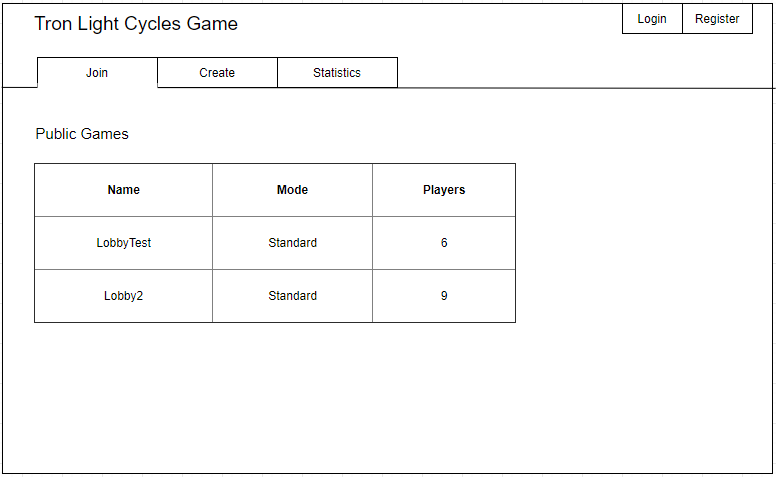
\includegraphics[scale=0.6]{figures/Mockup_Join.png}
    	\caption{Mockup Join}
    	\label{fig:MockupJoin}
    \end{figure}
    \subsubsection{Zuverlässigkeit}
    Wir können mit Sicherheit sagen, dass unsere Applikation nicht sonderlich anfällig für Ausfälle ist. Da das Spiel nur eine geringe Leistung beansprucht, verringert das die Fehlerquellen enorm. Die Applikation ist auch Client abhängig. Das bedeutet, falls ein Spieler Verbindungsprobleme hat oder andere Schwierigkeiten, dann kann er verlieren. Die Lobby liegt auf dem Server, somit ist gewährleistet, dass falls der Spieler, welche die Lobby erstellt hat, Verbindungsprobleme hat, das Spiel weiterhin normal abläuft. Dies ist ebenso ein wichtiger Aspekt für uns, damit das Spiel reibungslos ohne Unterbrüche ablaufen kann.
    \subsubsection{Effizienz}
    Da wie bereits erwähnt das Spiel nur eine geringe Leistung beansprucht, ist die Effizienz gut und zuverlässig. Hier spielt leider auch wieder der Client eine Rolle. Da der Server und der Client in Verbindung stehen und der Client Verbindungsprobleme oder sonstige Verzögerungen hat, kommt es schnell zu kurzen Unterbrechungen für den Spieler. Dies ist kaum zu vermeiden.
    \subsubsection{Änderbarkeit (Wartbarkeit)}
    Die Applikation ist nur über den Browser erreichbar, dies macht die Wartbarkeit um einiges einfacher. Die diversen Browser müssen natürlich getestet werden und kompatibel sein. Die wichtigsten Browser sind Firefox, Google Chrome und Internet Explorer.  Das Testen neuerer Versionen der einzelnen Browser schliesst dies mit ein, um die Zuverlässigkeit weiterhin anbieten zu können.
    \subsubsection{Internationalisierung}
    In der ersten lauffähigen Version wird Englisch verwendet. Später sollen andere Sprachen folgen um grössere Reichweite zu generieren.
    \subsubsection{Designeinschränkungen}
    Wir benutzen React und Material UI für das Design, da Material UI bereits einige Bibliotheken, beziehungsweise vordefinierte  Bausteine zur Verfügung stellt. Da wir mit einer \Gls{SPA} arbeiten wird Routing vorerst nicht nötig sein.
    \subsubsection{Implementierungseinschränkungen}
    Um die Applikation so wartbar wie möglich zu behalten, wird alles so gut wie möglich mit Clean Code implementiert. Dies wird auch im späteren Verlauf des Implementierungsvorgangs immer wieder überprüft. Bei Git benutzen wir das \Gls{Continuous Integration} (CI), dies ermöglicht es uns nur kompilierbaren Code hinzuzufügen um einige Fehlerquellen bereits auszuschliessen.
    \subsubsection{Schnittstelleneinschränkungen}

    \subsection{Domänenmodell}
    \begin{figure}[H]
    	\centering
    	\makebox[\textwidth][c]{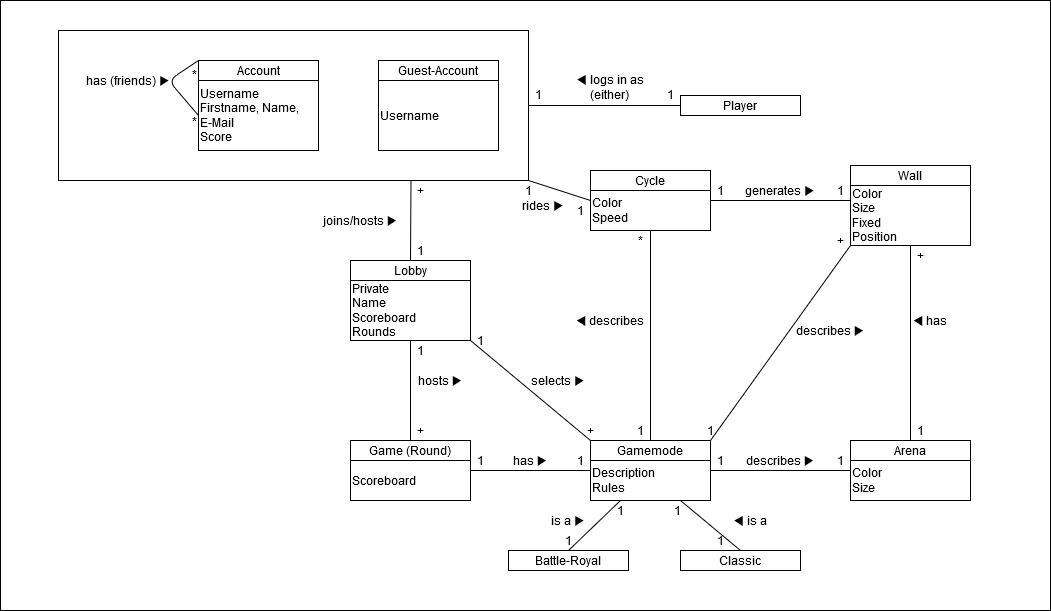
\includegraphics[width=1.1\textwidth]{figures/domain_model.png}}
    	\caption{Domänenmodell - Tron Licht-Motorräder Computerspiel}
    	\label{fig:DomainModel_TronLightCycles}
    \end{figure}
    \subsubsection{Login und Gast-Account}
    Der Spieler hat die Freiheit sich mit einem anonymen Gastkonto  oder mit einem registriertem Konto anzumelden. Der Spieler kann sich in der Applikation nicht mit beiden Kontoarten gleichzeitig identifizieren.

    \subsubsection{Spielemodi}
    Ein Spielmodus beeinflusst das Spiel, zwei Spielmodi werden schon implementiert sein. Im Spielmodus sind Eigenschaften der Licht-Motorräder und die Grösse der Arena definiert, so auch Spielablauf.

%%% END Analyse


%%%  Design
% Die wichtigsten Aspekte der gewählten Lösung sind zu dokumentieren:
%− Softwarearchitektur
%− Design-Klassendiagramm (DCD)
%− Ausgewählte Interaktionsdiagramme
%− Dokumentation wichtiger Architekturaspekte, Designentscheide und angewendeter Design Patterns
    \section{Design}

    \subsection{Softwarearchitektur}
    Abstrakter Überblick der Softwarearchitektur. \Gls{NGiNX} ist Webserver für den statischen Inhalt und \Gls{Reverse-Proxy} für GamerServer und Node.js Backend Anfragen, siehe \autoref{fig:Softwarearchitektur_abstract} .
        \begin{figure}[H]
        \centering
        \makebox[\textwidth][c]{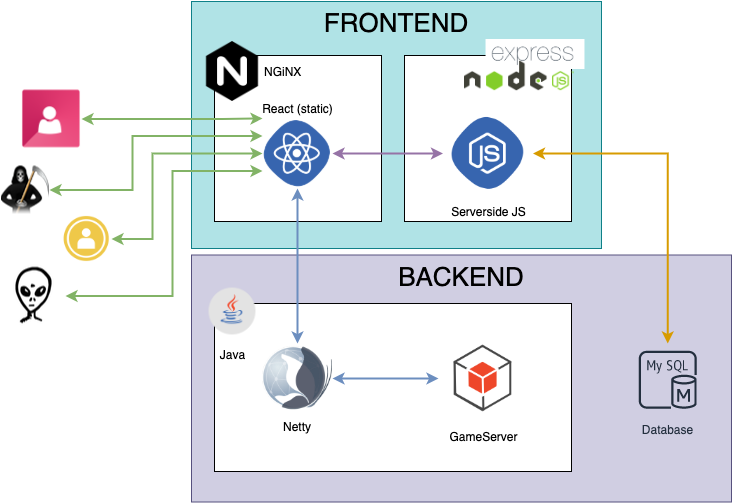
\includegraphics[width=0.9\textwidth]{figures/Tron_basic_architecture.png}}
        \caption{Abstrakte Softwarearchitektur - \Glspl{Microservice}}
        \label{fig:Softwarearchitektur_abstract}
    \end{figure}
    \newpage
    Detailierter Überblick aller Programme und Kommunikationswege.
    \begin{figure}[H]
        \centering
        \makebox[\textwidth][c]{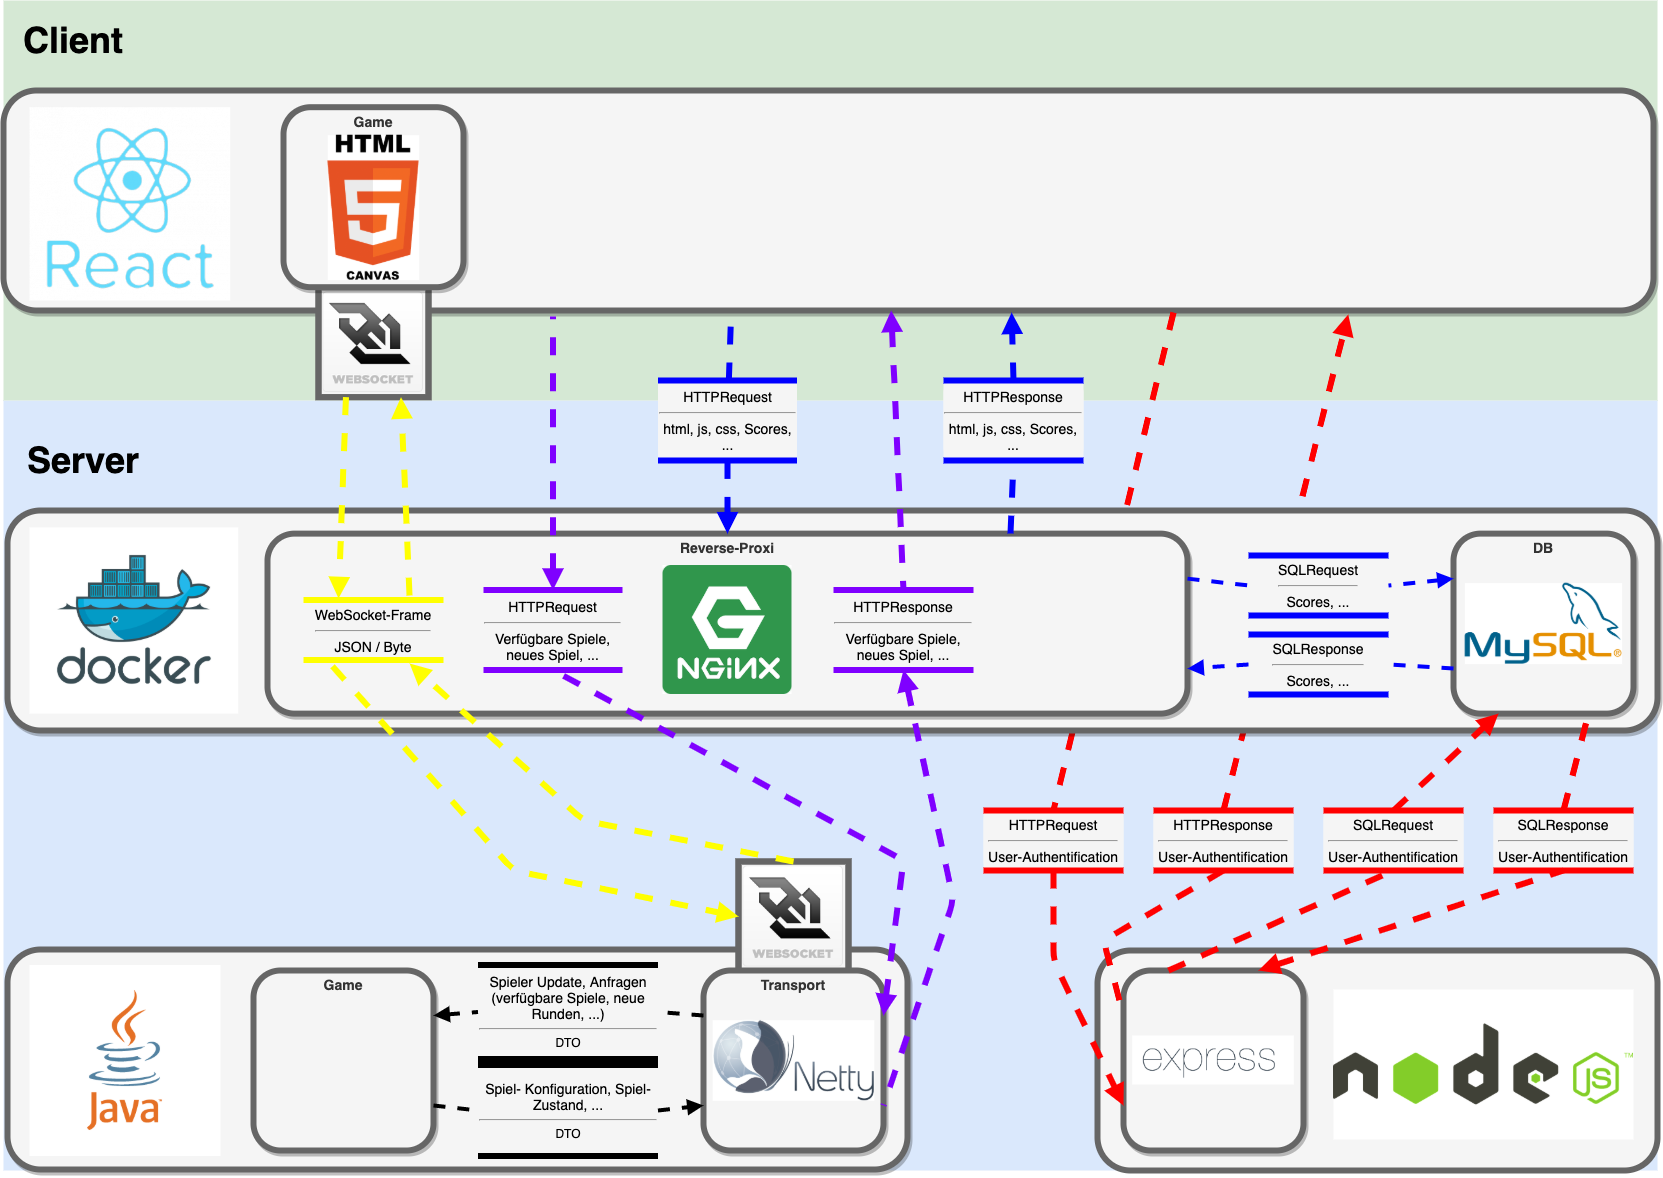
\includegraphics[scale=0.3]{figures/architecture-draft_v3.png}}
        \caption{Systemarchitektur}
        \label{fig:Systemarchitecture}
    \end{figure}

    \subsection{Interaktionsdiagramme}

    \subsubsection{SSD Hauptanwendungsfälle}
    Die zwei wichtigsten Hauptanwendungsfälle (siehe \ref{ssec:Hauptanwendungsfaelle} \nameref{ssec:Hauptanwendungsfaelle} ) sind in \ref{sssec:SSDFromProjectOutline} \nameref{sssec:SSDFromProjectOutline} dargestellt.

    \subsubsection{SSD \Gls{Websocket} Kommunikation zwischen Gameserver und Client}
    In \autoref{fig:SSDWS_GS_Client} sind die \Gls{Websocket} Mitteilungen ersichtlich die zweischen GameServer und Client verschickt werden. Der Ablauf kann folgendermassen erklärt werden:
    \begin{enumerate}
        \item \textit{Client1} - auf der linken Seite in Violet - baut eine Websocketverbindung zum \textit{GameServer} (in Grün) auf.
        \item Der \textit{GameServer} schickt dem \textit{Client1} eine eindeutige \inlinecode{bash}{clientId}.
        \item \textit{Client1} erstellt etwas später ein Spiel und die \inlinecode{bash}{createGame} Mitteilung wir an den \textit{GameServer} geschickt.
        \item Der \textit{GameServer} erstellt ein Spiel und schickt dem \textit{Client1} die \inlinecode{bash}{gameId}.
        \item Ein weiterer \textit{Client2} - auf der rechten Seite in Orange - hat in Zwischenzeit eine Websocketverbindung aufgebaut zum \textit{GameServer} und erhält eine \inlinecode{bash}{clientId} .
        \item \textit{Client1} ist nach dem erstellen des Spiels nun in der Lobby und erhält regelmässig den \inlinecode{bash}{lobbyState}
        \item \textit{Client2} tritt nun dem von \textit{Client1} erstellten Spiel bei mit \inlinecode{bash}{joinGame} und erhält darauf auch regelmässig den \inlinecode{bash}{lobbyState}. \textit{Client2} befindet sich nun auch in der Lobby.
        \item \textit{Client1} startet das Spiel mit der Mitteilung \inlinecode{bash}{startGame}.
        \item Der \textit{GameServer} schickt nun als erstes die \inlinecode{bash}{convasConfig}, dann den \inlinecode{bash}{initialGameState}, dann den \inlinecode{bash}{Countdown} und schlussendlich, in kurzen Intervallen, den \inlinecode{bash}{gameState}. Der \inlinecode{bash}{gameState} beeinhaltet die neu berechneten Positionen aller Spieler und somit beginnen diese sich zu bewegen.
        \item Die Spieler schicken - je nach Bedarf - eine Aktualisierung ihrer Richtung mit \inlinecode{bash}{updateDirection}.
        \item Der \textit{GameServer} schickt - je nach Bedarf - eine Benachrichtigung über das ausscheiden eines Spielers mit \inlinecode{bash}{playerDeath}.
        \item Nachdem alle Spieler ausgeschieden sind, wird eine \inlinecode{bash}{roundScores} Mitteilung an alle Spieler verschickt. Das Spiel ist nun beendet und alle Spieler sind wieder in der Lobby.
        \item Spieler können jederzeit das Spiel verlassen wenn diese \inlinecode{bash}{leaveGame} an den \textit{GameServer} schicken. \textit{Client1} und \textit{Client2} haben das Spiel verlassen.
        \item \textit{Client2} schliesst schlussendlich die Websocketverbindung zum \textit{GameServer}. Dies wird zum Beispiel ausgelöst, wenn das Browserfenster geschlossen wird.
    \end{enumerate}
    \begin{figure}[H]
        \centering
        \makebox[\textwidth][c]{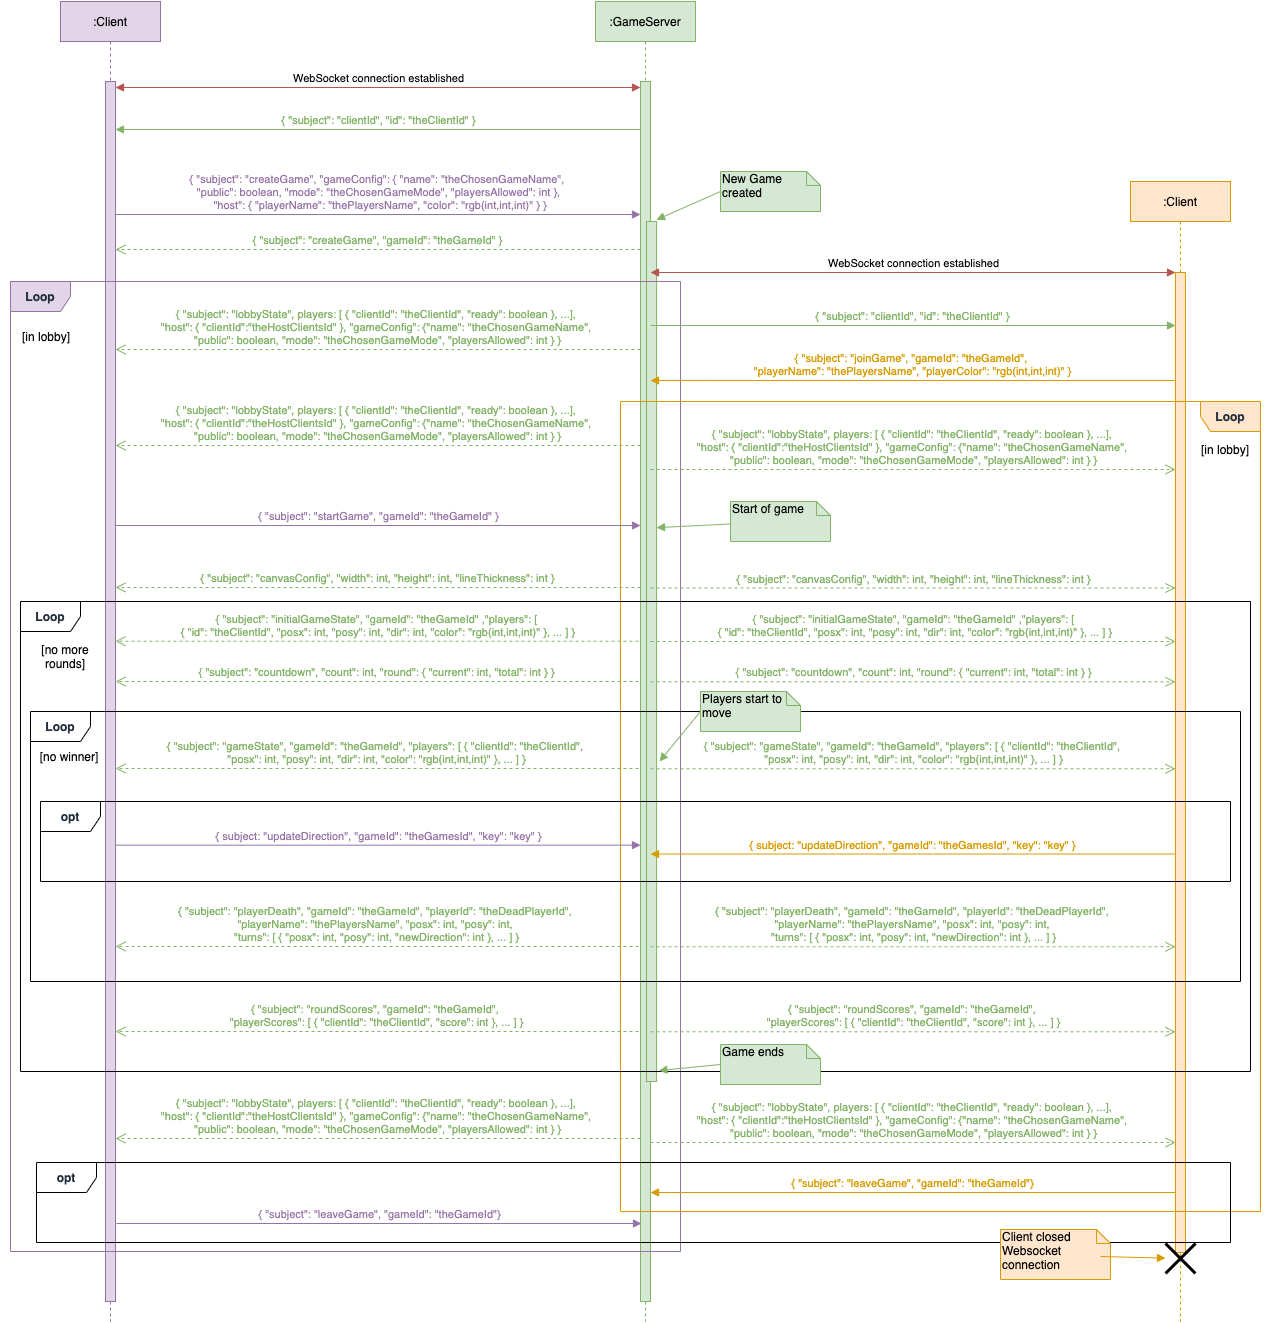
\includegraphics[scale=0.4]{figures/SSD_GameProcedure.png}}
        \caption{SSD - \Gls{Websocket} Kommunikation zwischen Gameserver und Client}
        \label{fig:SSDWS_GS_Client}
    \end{figure}

    \subsection{Designentscheide}

    \subsubsection{Kommunikation via Websocket}
    \Gls{Websocket} eignet  sich hervorragend für bidirektionale Client-Server-Kommunikation mit niedriger Latenz. Das ermöglicht eine beinahe  \quotes{Echtzeit}-Kommunikation zwischen dem Client (\Gls{Webbrowser}) und der Applikation. Die Implementation ist sehr einfach gelöst und gut dokumentiert. Zusätzlich wird \Gls{Websocket} von fast allen \Gls{Webbrowser} unterstützt. Aus diesen Gründen, ist \Gls{Websocket} für unsere Tron-Licht-Motorräder-Applikation die perfekte Lösung für den schnellen Datenaustausch während dem Spiel.

    \subsubsection{Gameserver  (Java)}
	Der Gameserver ist in vier Module aufgeteilt. Die strikte Modularisierung unter Verwendung von Java 9 Modules garantiert eine schwache Kopplung, wodurch die einzelnen Komponenten losgelöst voneinander implementiert werden konnten. Es existieren die Module Appmain (A), Transport (T), Game (G) und Middleman (M). Nachfolgend ein UML-Diagramm, das die Modul-Abhängigkeiten abbildet.

	\begin{figure}[H]
    	\centering
    	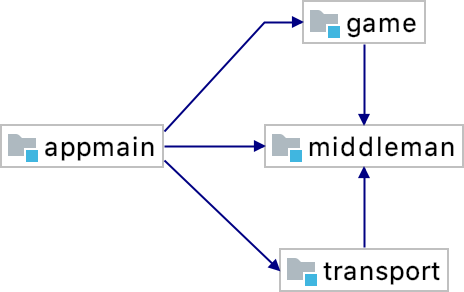
\includegraphics[scale=0.5]{figures/gameserver-uml/modules.png}
    	\caption{UML - Module des Gameservers}
    	\label{fig:UMLModule}
    \end{figure}

	\paragraph{Appmain (A)}
	Dieses Modul dient lediglich als Eintrittspunkt des Gameservers. Es beinhaltet die Main-Klasse, die die Hauptkomponenten der Module T, G und M initialisiert. Nachfolgend das Klassendiagramm zum Modul Appmain.

	\begin{figure}[H]
    	\centering
    	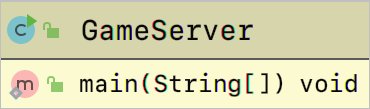
\includegraphics[scale=0.4]{figures/gameserver-uml/appmain-classes.png}
    	\caption{UML Klassendiagramm - Gameserver Modul Appmain}
    	\label{fig:UMLModulAppmain}
    \end{figure}

    \paragraph{Transport (T)}

	Das Modul Transport kümmert sich um den bidirektionalen Datenaustausch zwischen dem Gameserver und den Clients. Um einen kontinuierlichen Austausch gewährleisten zu können, werden zuverlässige Client-Server-Verbindungen mittels \Gls{Websocket}s aufgebaut. Ein Client sendet darüber die bei ihm auftretenden Events im Spiel wie zum Beispiel eine Richtungsänderung. Über das Modul M gibt das Modul T die erhaltenen Informationen an das Modul G weiter. Der Webserver wurde mit Hilfe von \Gls{Netty} implementiert. Das Klassendiagramm zum Modul T ist nachfolgend ersichtlich.

	\begin{figure}[H]
    	\centering
    	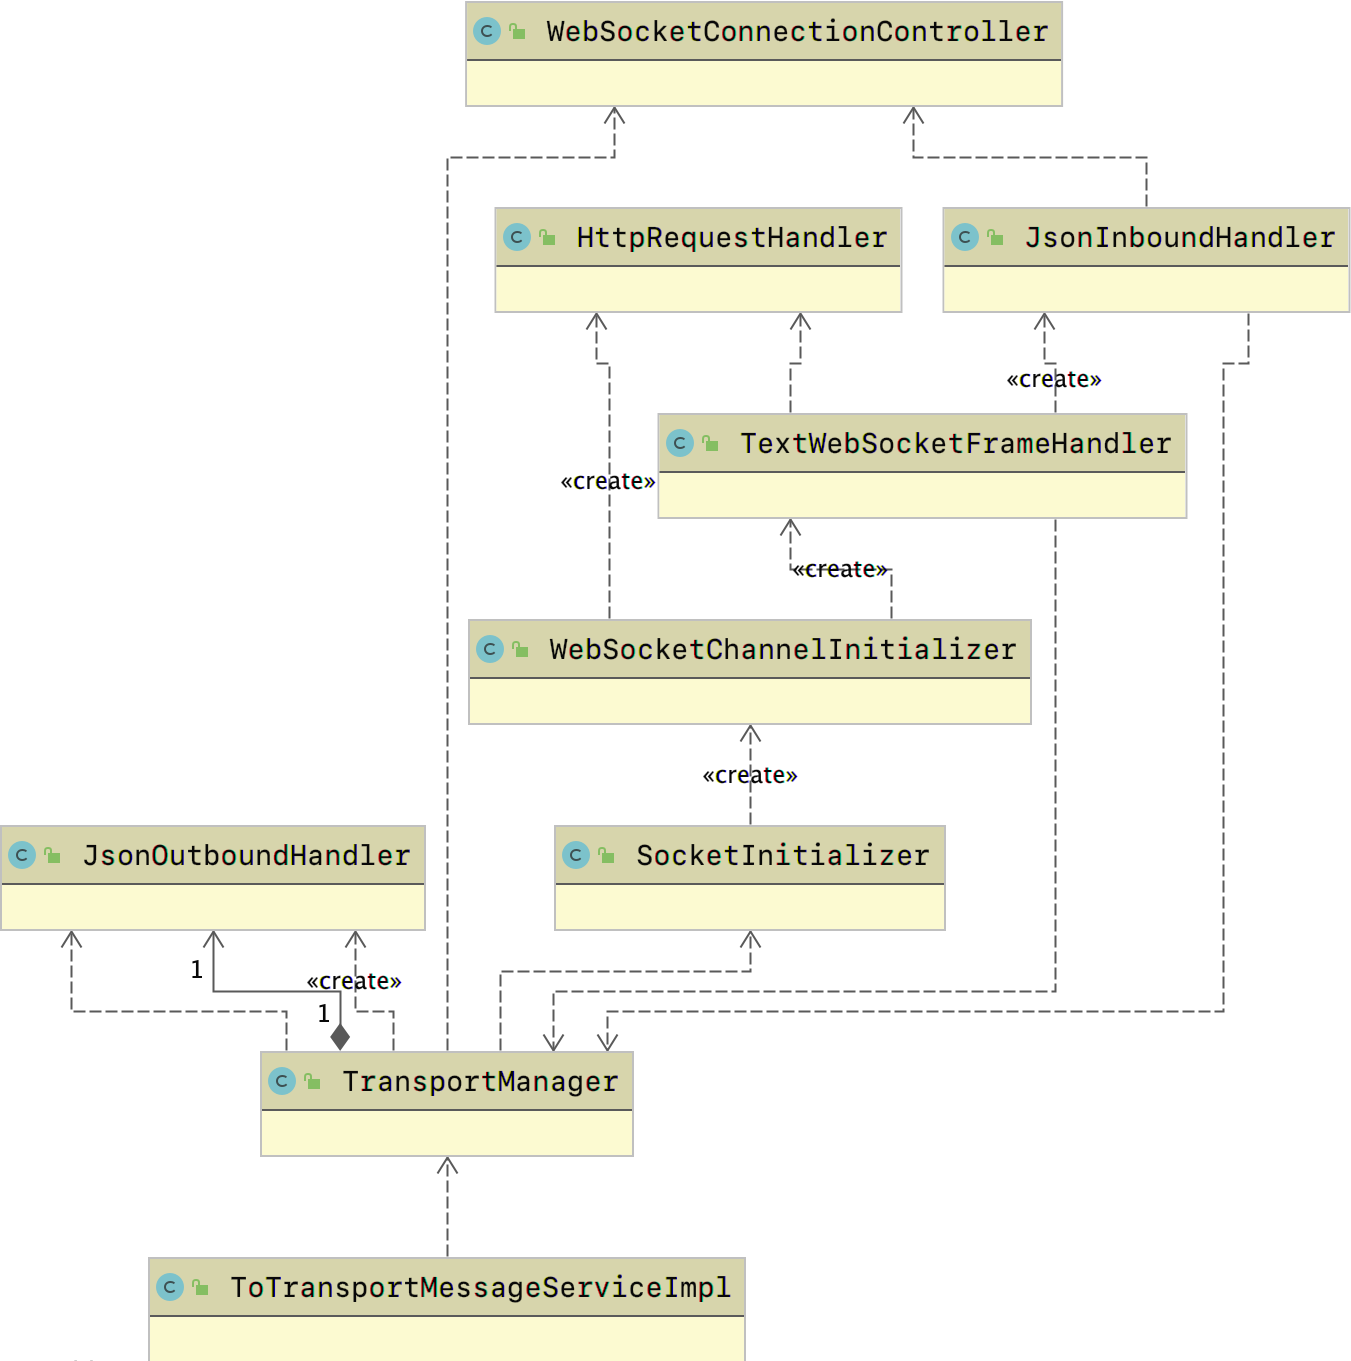
\includegraphics[scale=0.3]{figures/gameserver-uml/transport-classes.png}
    	\caption{UML Klassendiagramm - Gameserver Modul Transport}
    	\label{fig:UMLModulTransport}
    \end{figure}

	\paragraph{Middleman (M)}

	Das Modul Middleman wird benötigt, um eine zirkuläre Abhängigkeit zwischen den Modulen T und G zu vermeiden. Die gesammte Kommunikation von T und G erfolgt über M, deswegen auch der Name "Middleman". Technisch funktioniert dies folgendermassen: Wie im nachfolgenden Diagramm ersichtlich, definiert das Modul T Nachrichten-Objekte, die jeweils von der Klasse InAppMessage erben. Da T und G das Modul Middleman kennen, können die von M definierten Nachrichten-Objekte von T und G instanziert werden. Sendet das Modul T oder G eine Nachricht, wird durch Anwendung des Design-Patterns Inversion of Control erreicht, dass das Empfänger-Modul die Nachricht bearbeitet. Hierfür werden in M die Services ToTransportMessageService und ToGameMessageService definiert und die dazugehörigen Service-Providers in G und T implementiert.

	\begin{figure}[H]
    	\centering
    	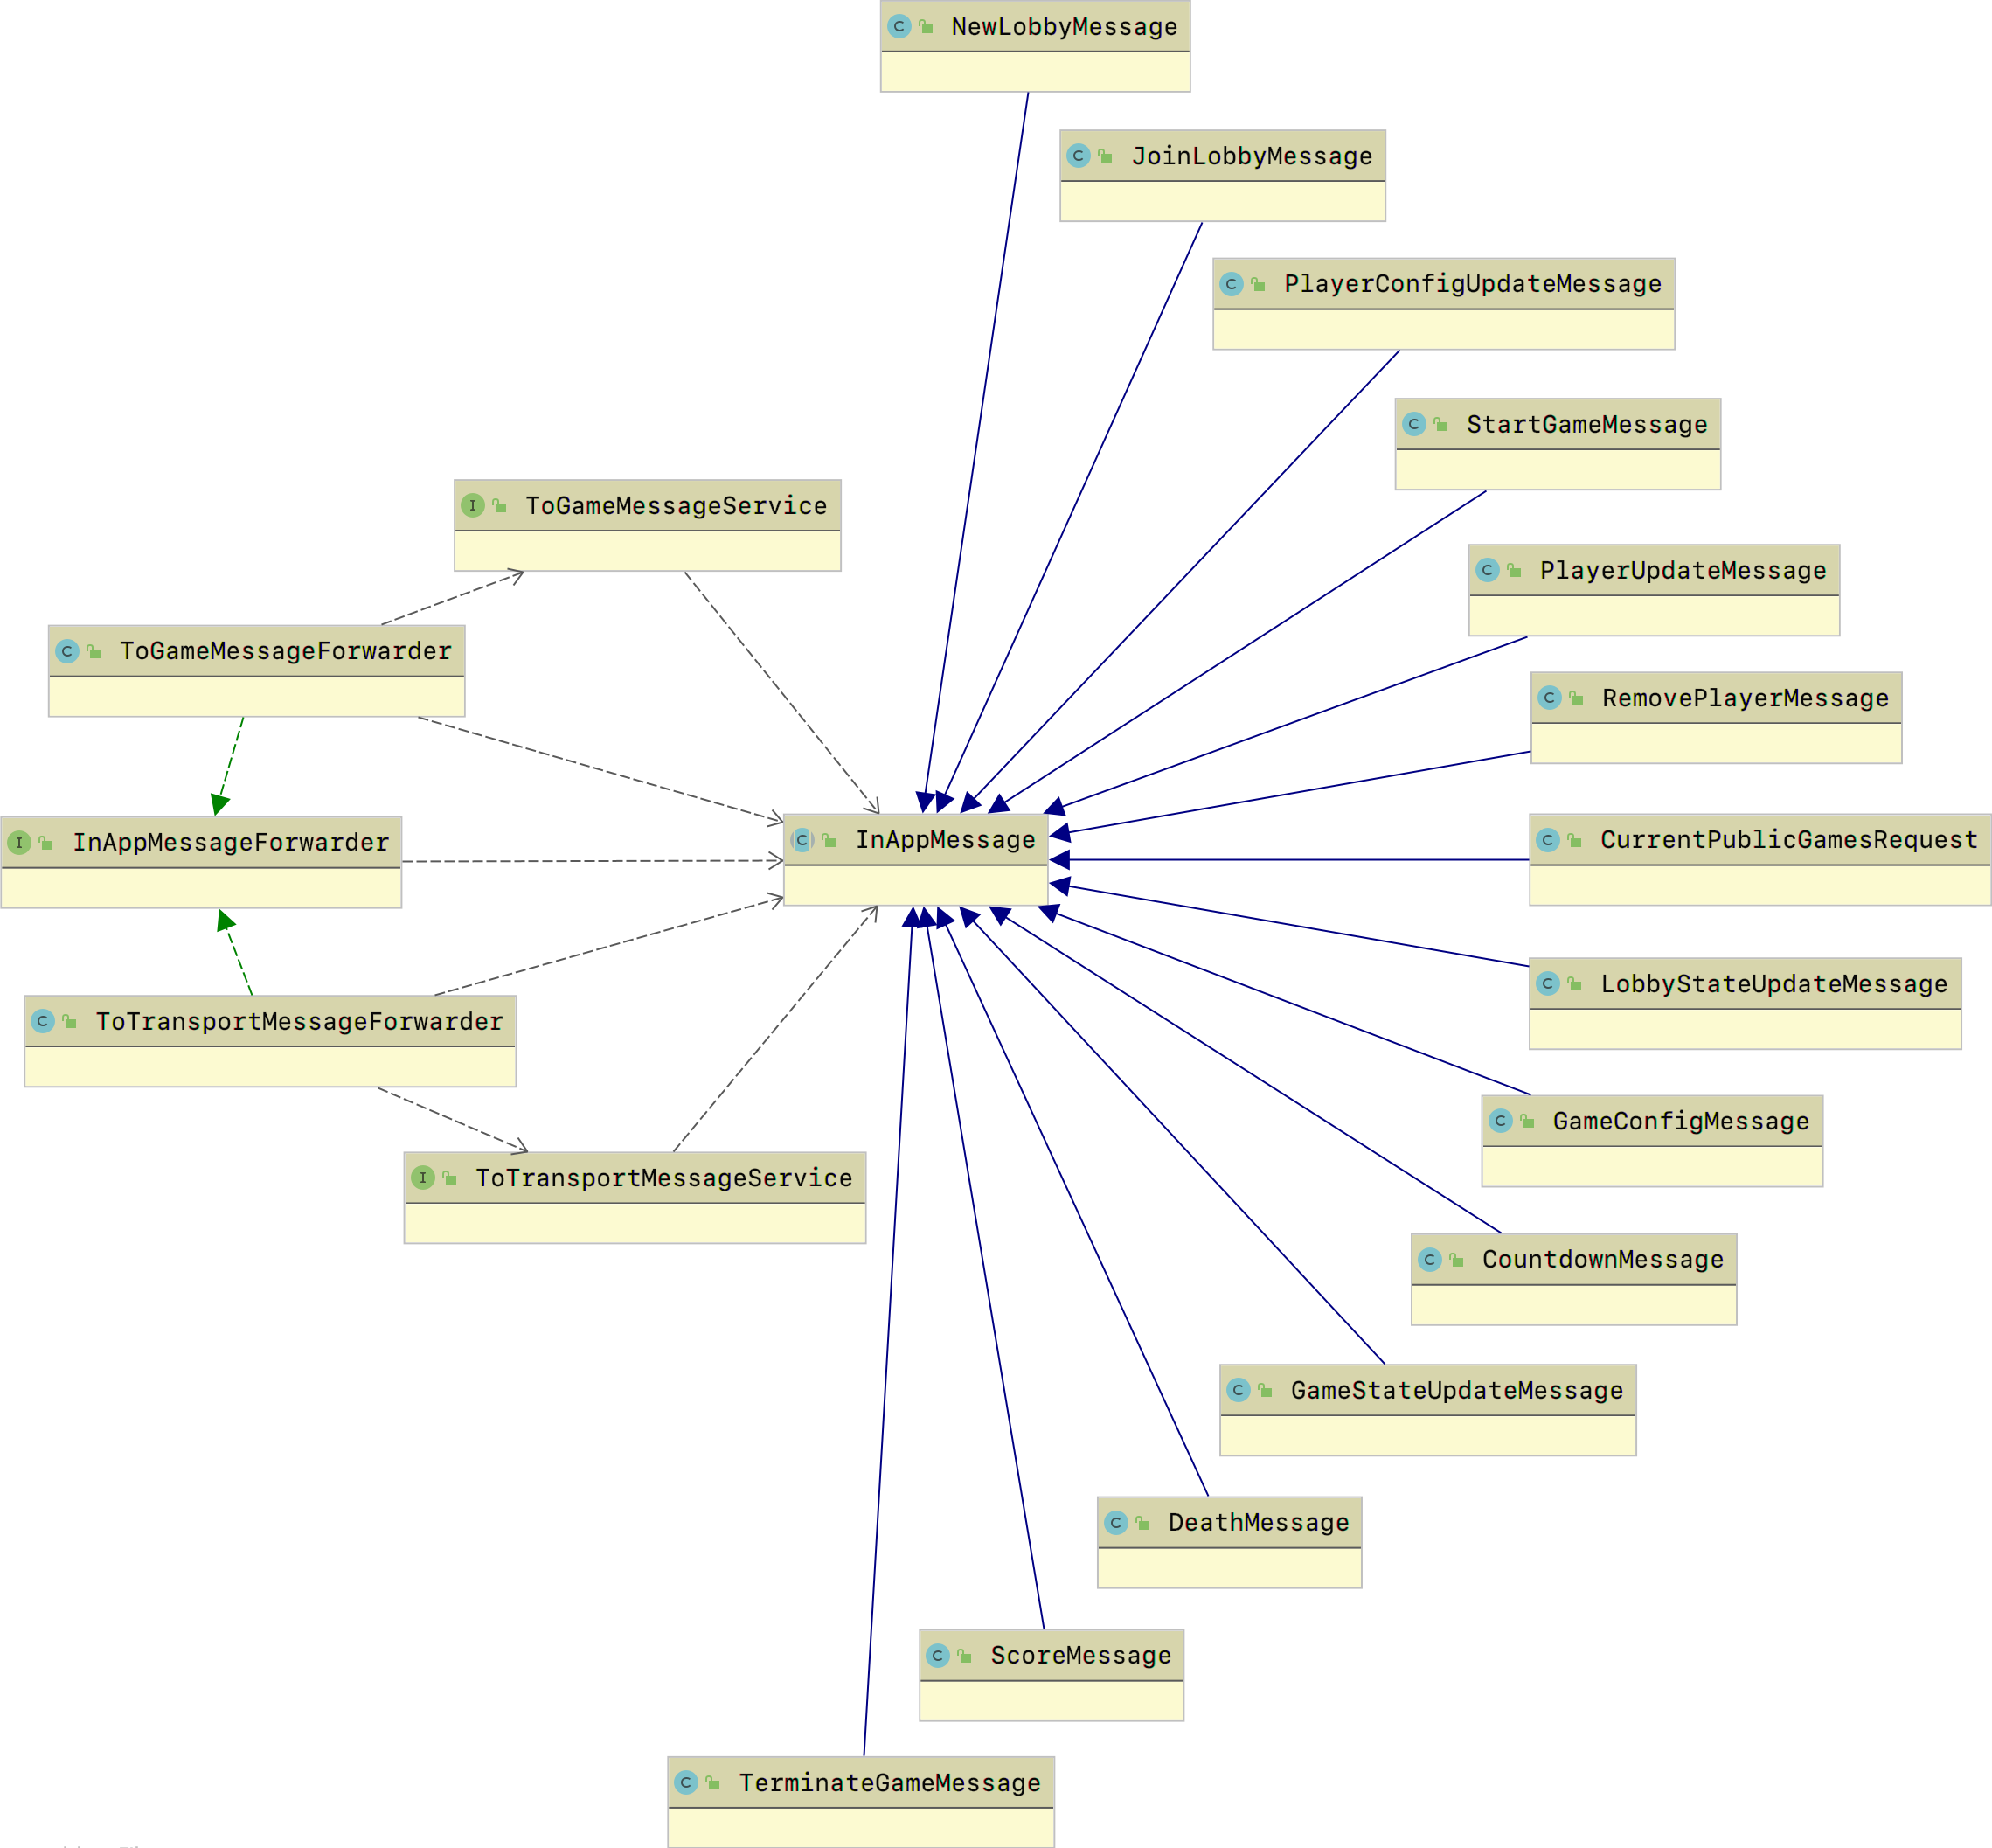
\includegraphics[scale=0.2]{figures/gameserver-uml/middleman-classes.png}
    	\caption{UML Klassendiagramm - Gameserver Modul Middleman}
    	\label{fig:UMLModulMiddleman}
    \end{figure}

    \paragraph{Game (G)}
	Das Modul Game beinhaltet das Management der \Gls{Lobby} und Spiellogik der einzelnen Spielmodi. Das Modul G leitet jeweils der Wechsel vom \Gls{Lobby}-Modus in den Spielmodus ein, berechnet auf verschiedenen Threads die Spielstände der laufenden Spiele und schickt diese über M an T. Nach Beenden einer Runde berechnet es die Scores der einzelnen Spieler und versendet auch diese. Nachfolgend das UML-Klassendiagramm zum Modul Game.

	\begin{figure}[H]
    	\centering
    	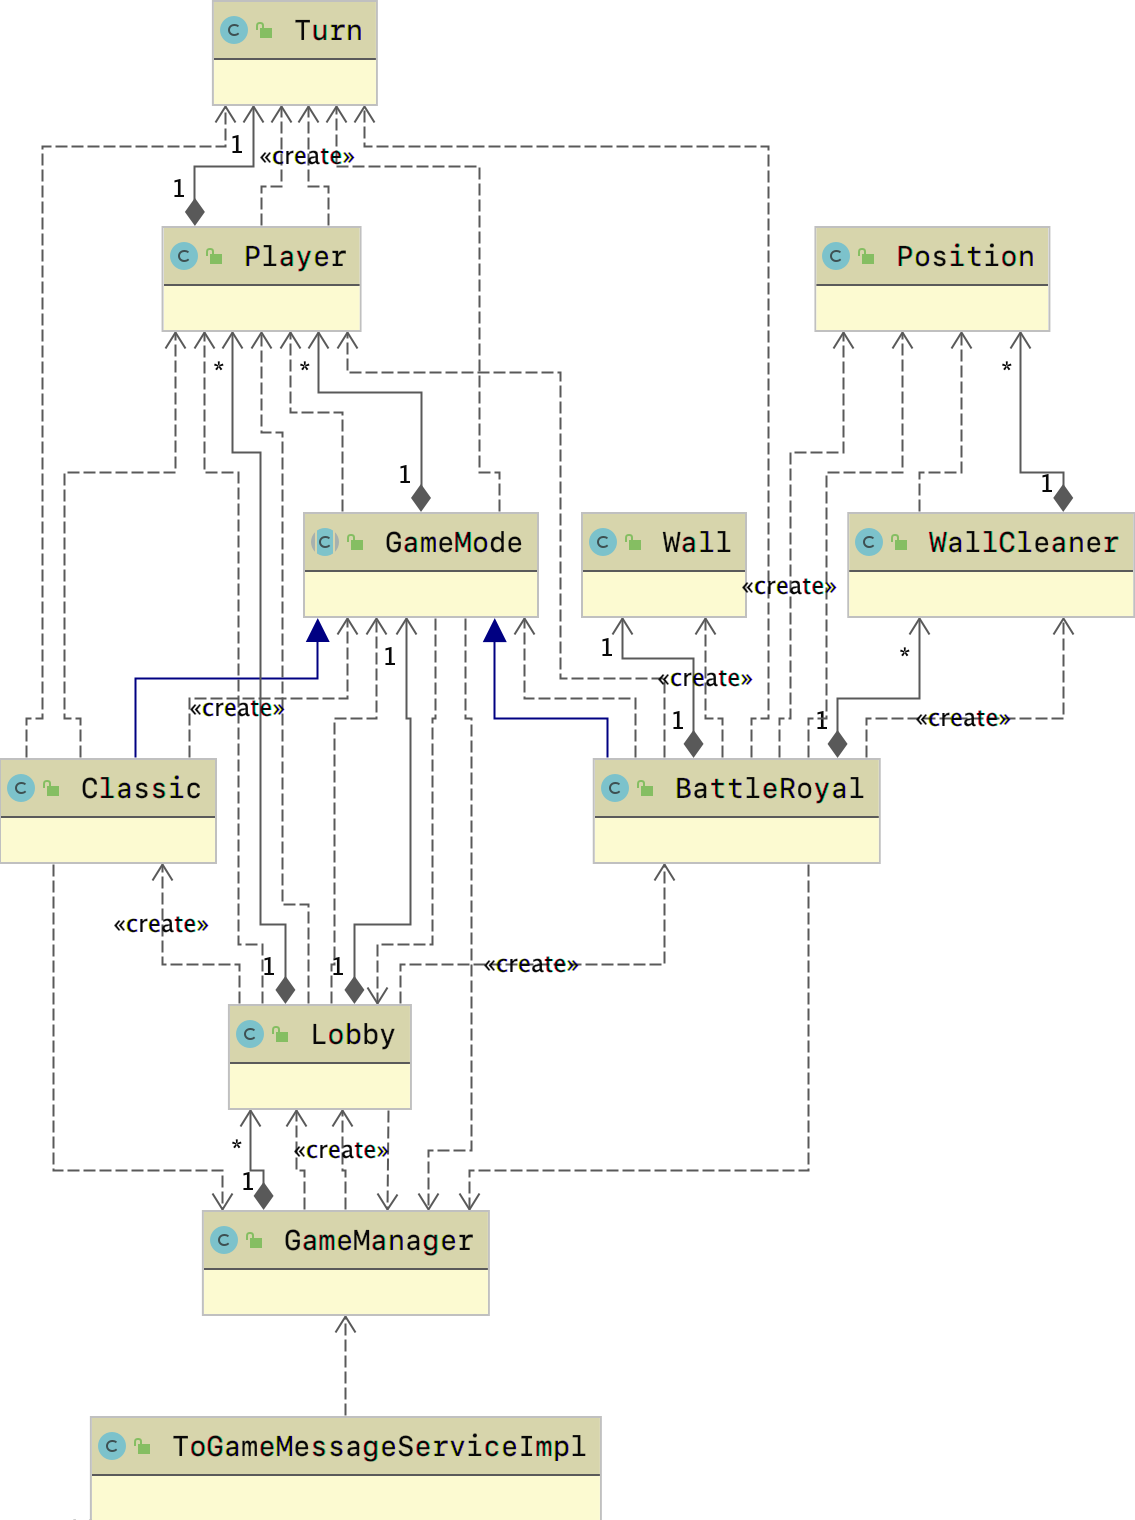
\includegraphics[scale=0.3]{figures/gameserver-uml/game-classes.png}
    	\caption{UML Klassendiagramm - Gameserver Modul Game}
    	\label{fig:UMLModulGame}
    \end{figure}

    \subsubsection{Rendering}
    Die ganzen virtuellen Objekte müssen am Ende auf dem Bildschirm des Users angezeigt werden. Dies kann über mehrere Arten erreicht werden und auch in unserem Projekt verwenden wir für jeden Spielmodus einen anderen Algorithmus. Bei beiden wird ein \Gls{Canvas} verwendet, dieses wird aber jeweils anders aufgebaut.

    \paragraph{Classic}
    Im Classic Modus sieht jeder Spieler das ganze Spielfeld, daher sind die einzigen bewegenden Elemente die Licht-Motorräder. Die neusten Positionen der Licht-Motorräder bekommt der Client vom GameServer 60 mal in der Sekunde aktualisiert über. Der Browser muss dann nur an der neuen Position die richtige Farbe setzen. Bis das Spiel fertig gespielt ist und das ganze \Gls{Canvas} zurückgesetzt wird.

    \paragraph{BattleRoyale}
    Beim BattleRoyale Modus kann das \Gls{Canvas} nicht mehr als Bildspeicher verwendet werden. Da der Spieler nur einen Teil des ganzes Spielfeld sieht und sein Licht-Motorrad zentral im Bild erscheinen sollte, bewegt sich alles ausser der eigener Spieler. Um dies korrekt darzustellen wurden zwei Designänderungen gegenüber dem Classic Renderer vorgenommen. Das Bild muss jedes Mal komplett neu gezeichnet werden und die Kamera muss sich der Position des Licht-Motorrads anpassen. Da das Bild immer neu gezeichnet werden muss, kann also das \Gls{Canvas} nicht mehr als Speicher für die vergangenen Schritte oder im Rahmen vom Spiel von den Wänden benutzt werden. Glücklicherweise sind es im BattleRoyale keine fixen Wände sondern dienen eher einem Schweif. Dieser Schweif hat eine fixe Länge und nur die Positionen bis zur Länge müssen gespeichert werden.

    \begin{figure}[H]
    	\centering
    	\makebox[\textwidth][c]{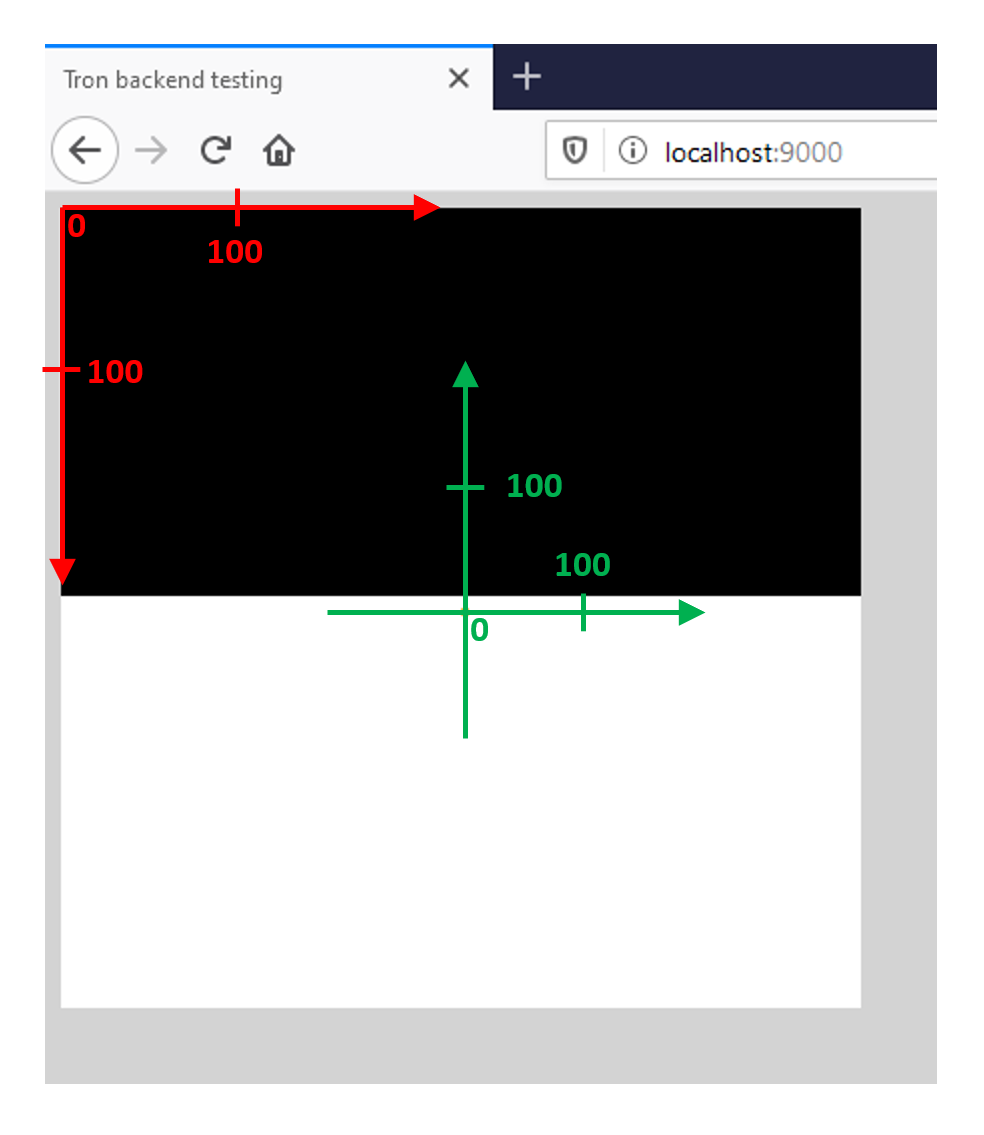
\includegraphics[scale=0.5]{figures/battleroyale_rendering_coordinates.png}}
    	\caption{BattleRoyale - Koordinatenansicht}
    	\label{fig:BattleRoyale_Coordinates}
    \end{figure}


	Die grünen Koordinaten sind relativ des Licht-Motorrads. Dort wo das Motorrad steht ist die Koordinate (x:0/y:0). Das Canvas arbeitet aber mit den roten Koordinaten und der GameServer versendet wiederum Koordinaten die sich auf das Spielfeld referenzieren. Die korrekte X-Koordinate wird nun so berechnet:

	\begin{center}
	\textit player.x - client.x + ( width / 2 )
	\end{center}

	Wir nehmen die X-Koordinate eines Mitspielers subtrahieren sie mit der X-Koordinate vom spielender Spieler und addieren die Hälfte der Breite des zusehenden Spielfeldes hinzu. Das gleiche gilt für die Y-Koordinate. Wenn nun alle Spieler und Wände berechnet sind, können wir das Bild richtig anzeigen.

	\begin{figure}[H]
		\centering
		\makebox[\textwidth][c]{
\includegraphics[scale=0.5]{figures/battleroyale_rendering1.png} 
\includegraphics[scale=0.5]{figures/battleroyale_rendering2.png}}
		\caption{BattleRoyale - Screenshots}
		\label{fig:BattleRoyale_screenshots}
	\end{figure}

	Zwei Screenshots, links zeigt der Stand nach den ersten 5 Schritten, rechts zeigt der Stand nach 15 Schritten. Zusehen ist, wie das Licht-Motorrad im Zentrum des Bildes bleibt, obwohl es sich nach unten bewegt.

    \subsubsection{User Interface mit React JavaScript library}
    Um die Benutzeroberfläche zu bauen, haben wir \Gls{React} eingesetzt. Die erlaubt es uns sogenannte Komponenten einzusetzen, die an diversen Orten wiederverwendet werden können.

    \subsubsection{Material-UI React Components}
    Die Material-UI Sammlung (\url{https://material-ui.com/}) der \Gls{React} Komponenten erlaubte uns, fertige Komponenten einzusetzen, ohne diese selber entwickeln zu müssen. Dies bedeutet eine schnellere Entwicklung mit schon ausgereiften Komponenten welche schon in etlichen anderen Applikationen eingesetzt wurden.

%%% END Design

%%% Implementation
%Die wichtigsten Informationen zur Implementation der Lösung (Packages, etc.) sowie die durch- geführten Tests sind hier zu dokumentieren:
%− Testkonzept: Zusammenfassung des gemachten Tests (Unit-, Integrations- und System- tests) und Testresultate
%− Installationsanleitung
%− Code-Dokumentation
%• Der vollständige Quellcode (inkl. Unit-Tests) wird in elektronischer Form abgegeben (auf OLAT im Team-Ordner als ZIP-File).
%• Jede Klasse und alle öffentlichen Methoden und Attribute müssen (kurz) mittels JavaDoc dokumentiert werden. Der fertige JavaDoc-Kommentar muss ebenfalls (elektronisch) ab- gegeben werden.
    \section{Implementation}

    \subsection{Testkonzept}
    Unser System besteht aus mehreren Programmiersprachen und diese werden auf verschiedenen Systemen eingesetzt. Das als ganzes zu testen braucht es eben so viel Programmierarbeit. Wir haben uns daher auf das mögliche konzentriert und hauptsächlich Unit-Tests angewendet und das ganze System von Hand getestet.

    \subsubsection{Unit Tests}
	Beim Gameserver wird das fast das ganze Modul Game mit Unit Tests getestet. Hauptsächlich wird geprüft, dass die korrekten Werte gesetzt, zurück gegeben und berechnet werden.

    \subsubsection{Integration Tests}

    \subsubsection{Systemtests}
    % read: https://www.enzyklopaedie-der-wirtschaftsinformatik.de/lexikon/is-management/Systementwicklung/Hauptaktivitaten-der-Systementwicklung/Software-Implementierung/Testen-von-Software/Systemtest/index.html

    \subsection{Continuous integration}
    Um  die kontinuierliche Integration \Gls{Continuous Integration} zu gewährleisten und für ein schnelles Feedback und bessere Codequalität, haben wir Github Actions (\url{https://github.com/features/actions}) eingesetzt. Der Workflow ist in \autoref{lst:GHAction} ersichtlich  und ist in zwei Teile (jobs) gegliedert und führt - abstrakt erklärt - folgende Schritte aus:

    \begin{itemize}
        \item \inlinecode{bash}{maven_java}: Der Java Code wird in der Java Version 11, 12 und 13 kompiliert und danach getestet.
        \item \inlinecode{bash}{npm_react}: Das React Frontend wird in der Node.js Version 8.x, 10.x und 12.x installiert und danach getestet.
    \end{itemize}

    \lstinputlisting[language=bash,label={lst:GHAction}, caption=Github Action workflow]{listings/CI_gh_actions.yml}
    \vspace{.5cm}
    % github actions => https://github.com/features/actions

    \subsection{Installationsanleitung}
    % pre-build and  docker-compose
    Um  die Tron Licht-Motorräder Applikation zu installieren, haben  wir uns für ein auf \Gls{Docker}-Container basierendes \Gls{Docker-Compose}-Setup entschieden. Somit lässt sich die Applikation einfacher verteilen/skalieren und ist modular - in sogenannten \Glspl{Microservice} - aufgebaut.

    \subsubsection{Voraussetzungen}
    Um die Applikation Schritt für Schritt installieren zu können, müssen folgende Voraussetzungen auf dem Zielsystem erfüllt sein.
    \begin{itemize}
        \item Software:
            \begin{itemize}
                \item Docker Community Edition (Docker CE) - \url{https://docs.docker.com/get-docker/}
                \item Node.js (v8.x oder neuer) \& npm  - \url{https://www.npmjs.com/get-npm}
            \end{itemize}
        \item Hardware :
            \begin{itemize}
                \item Mindestens 2 CPU Cores
                \item Mindestens 1024 MB RAM
            \end{itemize}
    \end{itemize}

    \subsubsection{Installationsschritte}
    Die einzelnen Schritte um die Applikation zu installieren:
    \begin{enumerate}
        \item Letzen Release der Applikation herunterladen: \url{https://github.com/22phuber/tron-light-cycles/releases}
        \item In den Projektordner wechseln: \inlinecode{bash}{/pfad/zum/projekt/tron-light-cycles/docker}
        \item Pre-Build Skript ausführen: \inlinecode{bash}{./pre-build.sh}
        \item \Gls{Docker}-Container bauen: \inlinecode{bash}{docker-compose build --no-cache}
        \item \Gls{Docker-Compose}-Setup starten: \inlinecode{bash}{docker-compose up -d}
        \item \url{http://localhost/}im Browser öffnen
    \end{enumerate}


    \subsection{Code-Dokumentation}
    Generieren der Javadoc. \Gls{Apache Maven} muss auf dem Systems installiert sein.
    \begin{enumerate}
        \item In den Projektordner wechseln: \inlinecode{bash}{/pfad/zum/projekt/gameserver}
        \item \inlinecode{bash}{mvn javadoc:aggregate}
    \end{enumerate}

%%% END Implementation


%%% Resultat
%Die Projektresultate sind kurz zusammenzufassen und in Bezug auf die ursprüngliche Projek- tidee zu stellen:
%− Zusammenfassung der erreichten Ziele
%− Offene Punkte
%− Ausblick auf mögliche Weiterentwicklungen
    \section{Resultat}

    \subsection{Erreichte Ziele}
    Die Ziele, welche wir uns gesetzt haben, konnten wir erreichen. Das Unterfangen hat jedoch mehr Aufwand erfordert als ursprünglich gedacht. Die Schwierigkeit lag darin alles einfach zu halten. Sobald ein Problem auftrat, wurde uns klar, es fehlen noch 5 weitere Dinge. \newline
    \newline
    \noindent Hinsichtlich des Projekts konnten wir folgende Ziele erreichen.

	\begin{itemize}
		\item Anmeldung/Registrierung
		\item Gastanmeldung
		\item Lobby erstellen
		\item Lobby beitreten
		\item Private und public Lobbys
		\item Komplexer Lobbymechanismus
		\item Spieler einladen mit Browser-Link
		\item Spielstart und spielen über das Netzwerk
		\item Akzeptable Latenz
		\item Zentraler Server
		\item Standardmodus und Battle Royale Modus
	\end{itemize}
    Die Gruppe hat zusätzlich viel Wissen durch neue Technologien gesammelt. Trotz unbekannter Hürden, welche dadurch verursacht wurden.

    \subsection{Offene Punkte}
    Die wichtigsten vordefinierten Ziele konnten erreicht werden. Folgende Punkte sind jedoch noch offen bzw. hinzugekommen beim Tests und Nutzung der Applikation.

	\begin{itemize}
        \item Backend:
            \begin{itemize}
                \item \textit{Node.js}: Speichern der erreichten Punkte in der Datenbank
                \item \textit{Node.js}:  Api Endpoint und Evaluierung des Authentifizierungstokens (JWT) für \quotes{My Account} Anfragen.
            \end{itemize}
       \item Frontend:
            \begin{itemize}
                \item \textit{React}: \quotes{My Account} Implementation
                \item \textit{React}: Speichern des Authentifizierungstokens (JWT) im Memory
                \item \textit{React}: \Glspl{Sprite} einsetzen, z.B. für das \quotes{Licht-Motorrad} im \Gls{Canvas} (HTML-Element)
                 \item \textit{React}: Implementation Werbeflächen
            \end{itemize}
        \item Applikation:
            \begin{itemize}
                \item Belastungstests. Wieviele Spieler können gleichzeitig, mit akzeptabler Latenz und Framerate, spielen?
            \end{itemize}
	\end{itemize}

    \subsection{Weiterentwicklungsmöglichkeiten}
    Damit das Spiel einen länger anhaltenden Spielspass gewähren kann, sowie zusätzlichen Profit generieren kann sind bereits einige Punkte notiert.

    \begin{itemize}
	    \item Aufzeichnen und Auswertung von Scores, Levels und Statistiken
	    \item In App-Käufe, wie z.B das Kaufen eines neuen Licht-Motorrads
	    \item Hindernisse im Spiel
	    \item Features, wie z.B Schiessen oder ein Speed Up
		\item Ein Modus, bei welchem sich das Spielfeld immer weiter verkleinert und die Linie hinter dem Spieler verschwindet.
	\end{itemize}

	Diese sind nur einige Weiterentwicklungsmöglichkeiten. Wir sind der Meinung, dass dieses Projekt sehr viel Potenzial für langanhaltenden Erfolg und unbegrenzte Weiterentwicklungsmöglichkeiten hat.
%%% END Resultat

%%%  Appendix
% - Projektmanagement
%Beschreibung des Vorgehens/Methodik (Phasen-/Iterationsplan). Zusammenfassung der tatsächlichen Aufwände mit den geplanten Aufwänden pro Iteration und insgesamt. Begrün- dung von signifikanten Abweichungen.
%− Verzeichnisse
%• Literatur-, Abbildungs-, Tabellenverzeichnis
%• Glossar
    \section{Appendix}

    \subsection{Projektmanagement}
    \begin{tabularx}{\textwidth}{X}
    	\toprule
    	Phase: \textbf{Inception} Iteration: \textbf{1} Woche: \textbf{1} Dauer: \textbf{2 Wochen}\\
    	\begin{compactitem}
    		\item Projektskizze erstellt.
    		\item Tools zusammengestellt.
    		\item Architektur erstellt.
    	\end{compactitem}\\
    	\toprule
    	\rowcolor{lightgray}
    	\textbf{Meilenstein 1} Woche: \textbf{2 Ende}\\
    	\rowcolor{lightgray}
    	\begin{compactitem}
    		\item \textbf{Vision definiert.}
    		\item \textbf{Geschäftsmodel definiert.}
    		\item \textbf{Anwendungsfälle definiert und Priorisierung vorgenommen.}
    		\item \textbf{Wichtigste nicht-funktionalen Anforderungen definiert.}
    	\end{compactitem}\\
    	\toprule
    	Phase: \textbf{Elaboration} Iteration: \textbf{2} Woche: \textbf{3} Dauer: \textbf{2 Wochen}\\
    	\begin{compactitem}
    		\item Softwarearchitektur festgelegt.
    		\item Domänenmodell erstellt.
    		\item Kernprozesse detaillierter definiert.
    	\end{compactitem}\\
    	\toprule
    	Phase: \textbf{Elaboration} Iteration: \textbf{3} Woche: \textbf{5} Dauer: \textbf{2 Wochen}\\
    	\begin{compactitem}
    		\item Serverseitige Datenbank Kommunikation.
    		\item Zusätzliche Anforderungen detaillierter festgelegt.
    		\item Entwicklung des Kernprozesses

    	\end{compactitem}\\
    	\toprule
    	\rowcolor{lightgray}
    	\textbf{Meilenstein 2} Woche: \textbf{6 Ende}\\
    	\rowcolor{lightgray}
    	\begin{compactitem}
    		\item \textbf{Alle Anforderungen stabilisiert.}
    		\item \textbf{Kern-Architektur implementiert und getestet.}
    	\end{compactitem}\\
    	\toprule
    	Phase: \textbf{Construction} Iteration: \textbf{4} Woche: \textbf{7} Dauer: \textbf{2 Wochen}\\
    	\begin{compactitem}
    		\item Anwendungsfälle 1, 2, 4 implementiert und getestet.
    	\end{compactitem}\\
    	\toprule
    	Phase: \textbf{Construction} Iteration: \textbf{5} Woche: \textbf{9} Dauer: \textbf{2 Wochen}\\
    	\begin{compactitem}
    		\item Anwendungsfälle 3, 5, 6, 7 implementiert und getestet.
    	\end{compactitem}\\
    	\toprule
    	Phase: \textbf{Construction} Iteration: \textbf{6} Woche: \textbf{11} Dauer: \textbf{2 Wochen}\\
    	\begin{compactitem}
    		\item Zusätzliches Testing und offene Probleme beheben
    	\end{compactitem}\\
    	\toprule
    	\rowcolor{lightgray}
    	\textbf{Meilenstein 3} Woche: \textbf{12 Ende}\\
    	\rowcolor{lightgray}
    	\begin{compactitem}
    		\item \textbf{System bereit für Produktion.}
    		\item \textbf{Bedienungsanleitung geschrieben.}
    	\end{compactitem}\\
    	\bottomrule
    \end{tabularx}

    \subsection{Iterationsplan}
    \begin{table}[H]
    	\caption{Iterationsplan}
        \begin{threeparttable}
    	   \begin{tabularx}{\textwidth}{l l l l l l X}

    	   	\toprule
    	   	Nr.\tnote{1} & S\tnote{2} & E\tnote{3} &  Soll\tnote{4}  & Ist\tnote{5} & MS\tnote{6} & Ziele \\
    	   	\toprule
    	   	Inception &&&& \\

    	   	1 & 19-02-20 & 04-03-20 & 73 & 102 & M1 & Vision definiert. Geschäftsmodell definiert. Anwendungsfälle definiert und Priorisierung vorgenommen. Wichtigste nicht-funktionalen Anforderungen definiert. Recherche zu Technologien angestellt. Projektskizze erstellen. \\

    	   	\toprule
    	   	Elaboration &&&& \\

    	   	2 & 04-03-20 & 25-03-20 & 62 & 74 & M2 & Weitere Technologie-Recherchen vornehmen. PoC Spiel spielen. Systemarchitektur definieren. Domänenmodell erstellen. Entwicklungsumgebung aufsetzen. Github Workflow, Continuous Integration einrichten. \\

    	   	3 & 25-03-20 & 08-04-20 & 126 & 159 & M2 & Implementation Systemarchitektur. Frontend Spiel spielen. Frontend Webseite Grundstruktur. Datenbank Setup und Anbindung. Gameserver modularisiert und stabilisiert. \\

    	   	\toprule
    	   	Construction &&&&\\

    	   	4 & 08-04-20 & 22-04-20 & 60 & 1 & M3 & Implementation Spielregeln. Implementation Spiel generieren. Implementation Spiel auswählen. \\

    	   	5 & 22-04-20 & 06-05-20 & 50 & 1 & M3 & \\

    	   	6 & 06-05-20 & 20-05-20 & 35 & 1 & M3 & \\
    	   	\toprule

    	   \end{tabularx}
        \begin{tablenotes}
            \item[1] Iterations Nummer.
            \item[2] Startdatum
            \item[3] Enddatum
            \item[4] Aufwand Soll [h]
            \item[5] Aufwand Ist [h]
            \item[6] Meilenstein
        \end{tablenotes}
       \end{threeparttable}


	\label{tab:Iterationsplan}
    \end{table}

    \subsection{Iterations-Assessment}
    Nachfolgend die Iterations-Assessments der vergangenen Iterationen.

    \subsubsection{Iteration 1}

    Zu Beginn sammelten wir viele Ideen für verschiedene Technologien. Dadurch haben wir viel Zeit damit aufgewendet, um die vorgeschlagenen Technologien zu studieren und die Vorteile, sowie die Nachteile abzuwägen.

    \begin{table}[H]
    	\caption{Iterations-Assessment: Iteration 1}
    	\begin{tabularx}{\textwidth}{X l l l}
    		\toprule
    		Arbeitspakete & Aufwand Soll [h] & Aufwand Ist [h] & Verantwortlicher \\
    		\toprule
    		Ideensammlung & 2 & 4 & alle \\
    		Vision Definition & 3 & 4 & Huber \\
    		Erarbeitung Geschäftsmodell & 3 & 4 & Iten \\
    		Definition Anwendungsfälle, Priorisierung & 10 & 15 & Akca \\
    		Definition Nichtfunktionale Anforderung & 5 & 5 & Iten \\
    		Projektskizze & 30 & 35 & alle \\
    		Recherche Technologie & 20 & 35 & alle \\
    		\bottomrule
    	\end{tabularx}
    	\label{tab:Iterations-Assessment: Iteration 1}
    \end{table}



    \subsubsection{Iteration 2}

    In der zweiten Iteration lag der Hauptfokus bei dem Festlegen der Grundarchitektur und wie die einzelnen Technologien zusammenspielen. Als nächstes wurde der grobe Ablauf des Spiels besprochen.

    \begin{table}[H]
    	\caption{Iterations-Assessment: Iteration 2}
    	\begin{tabularx}{\textwidth}{X l l l}
    		\toprule
    		Arbeitspakete & Aufwand Soll [h] & Aufwand Ist [h] & Verantwortlicher \\
    		\toprule
    		Sitzungen, Diskussionen & 5 & 7 & alle \\
    		Recherche Technologien & 8 & 12 & alle \\
    		Systemarchitektur Artifact & 3 & 4 & Holenstein \\
    		Domänenmodell & 5 & 5 & Akca \\
    		PoC Gameserver & 15 & 15 & Holenstein \\
    		Systemarchitektur Implementation & 10 & 12 & Huber \\
    		Entwicklungsumgebung & 5 & 6 & Iten \\
    		Projektmanagement Github & 5 & 5 & Huber \\
    		Github Actions Continuous Integration Setup & 6 & 8 & Huber \\
    		\bottomrule
    	\end{tabularx}
    	\label{tab:Iterations-Assessment: Iteration 2}
    \end{table}

    \subsubsection{Iteration 3}

    In der dritten Iteration haben wir uns genaue Gedanken darüber gemacht, wie die einzelnen Anwendungsfälle ablaufen. Des Weiteren kamen die ersten Frontendbeispiele und Kernprozesse zum Zug

    \begin{table}[H]
    	\caption{Iterations-Assessment: Iteration 3}
    	\begin{tabularx}{\textwidth}{X l l l}
    		\toprule
    		Arbeitspakete & Aufwand Soll [h] & Aufwand Ist [h] & Verantwortlicher \\
    		\toprule
    		Sitzungen, Diskussionen & 6 & 6 & alle \\
    		Recherche Technologien & 15 & 17 & alle \\
    		Ausformulierung Anwendungsfälle & 15 & 20 & Akca, Iten, Huber \\
    		Frontend Spiel spielen & 10 & 20 & Huber \\
    		Frontend Mockup & 5 & 7 & Iten \\
    		Frontend Webseite Implementation & 10 & 14 & Iten \\
    		Game Server Stabilisierung Kernarchitektur & 15 & 20 & Holenstein \\
    		Datenbank Setup, Anbindung & 10 & 10 & Akca \\
    		Projektmanagement Github & 5 & 5 & Huber, Akca \\
    		Lösungsarchitektur Dokument, Artifakte & 35 & 40 & alle \\
    		\bottomrule
    	\end{tabularx}
    	\label{tab:Iterations-Assessment: Iteration 3}
    \end{table}

    \subsubsection{Iteration 4}

    Während der vierten Iteration führten wir die Implementation der einzelnen Mechanismen des Spieles fort. Die Kommunikation zwischen Frontend und Backend wurde unter die Lupe genommen.

    \begin{table}[H]
    	\caption{Iterations-Assessment: Iteration 4}
    	\begin{tabularx}{\textwidth}{X l l l}
    		\toprule
    		Arbeitspakete & Aufwand Soll [h] & Aufwand Ist [h] & Verantwortlicher \\
    		\toprule
    		Sitzungen, Diskussionen & 2 & 2 & alle \\
    		Kommunikation Frontend/Backend & 10 & 12 & Holenstein, Akca \\
    		Gameserver Mechanismus Spiel & 19 & 25 & Holenstein, Akca \\
    		Datenbankanbindung & 5 & 4  & Iten \\
    		Projektmanagement Github & 3 & 2  & Huber \\
    		Frontend Anmeldung/Abmeldung/Gast & 5 & 8   & Iten \\
    		Frontend StateHandling & 10 & 12   & Huber \\
    		Frontend Designänderungen & 6 & 4 & Huber \\
    		\bottomrule
    	\end{tabularx}
    	\label{tab:Iterations-Assessment: Iteration 4}
    \end{table}

    \subsubsection{Iteration 5}

    In der fünften Iteration lag der Hauptfokus auf der Lobby. Zusätzlich wurden auch die Kommunikationsregeln zwischen Frontend und Backend finalisiert.

    \begin{table}[H]
    	\caption{Iterations-Assessment: Iteration 5}
    	\begin{tabularx}{\textwidth}{X l l l}
    		\toprule
    		Arbeitspakete & Aufwand Soll [h] & Aufwand Ist [h] & Verantwortlicher \\
    		\toprule
    		Sitzungen, Diskussionen & 4 & 5 & alle \\
    		Bedienungsanleitung & 10 & 11 & Iten \\
    		Kommunikation Frontend/Backend & 8 & 10 & Huber, Akca \\
    		Lobbymechanismus Backend & 15 & 21 & Holenstein, Akca \\
    		Projektmanagement Github & 3 & 5 & Huber \\
    		Frontend Lobby & 10 & 13 & Huber, Iten \\
    		\bottomrule
    	\end{tabularx}
    	\label{tab:Iterations-Assessment: Iteration 5}
    \end{table}

    \subsubsection{Iteration 6}

    In der letzten Iteration wurden noch auftretende Probleme behoben und der Battle Royal Modus eingebaut.

    \begin{table}[H]
    	\caption{Iterations-Assessment: Iteration 6}
    	\begin{tabularx}{\textwidth}{X l l l}
    		\toprule
    		Arbeitspakete & Aufwand Soll [h] & Aufwand Ist [h] & Verantwortlicher \\
    		\toprule
    		Sitzungen, Diskussionen & 5 & 4 & alle \\
    		Battle Royal Modus & 5 & 6 & Akca \\
    		Projektmanagement Github & 2 & 3 & Huber \\
    		Javadoc & 5 & 3 & Huber, Akca \\
    		Schlussbericht & 8 & 12 & alle \\
    		Bugfixing & 10 & 12 & Holenstein, Iten \\
    		\bottomrule
    	\end{tabularx}
    	\label{tab:Iterations-Assessment: Iteration 6}
    \end{table}

    \newpage
    \listoffigures
    \listoftables
    \printbibliography
    \printglossary
    \textit{Hinweis: Glossar-Referenznummern sind Seitennummern}

\newpage
\end{document}

